\documentclass{beamer}

\usepackage[english]{babel}
\usepackage{booktabs}
\usepackage{amsmath,amssymb,bm}
\usepackage{graphicx}
\usepackage{multicol}
\usepackage{tikz}
\usepackage[UKenglish]{isodate}

\makeatletter
\def\input@path{{../../theme/}}
\makeatother

\usetheme{cambridge}
\setbeamertemplate{navigation symbols}{}
\cleanlookdateon

\usetikzlibrary{arrows.meta,positioning,fit}

\graphicspath{
  {assets/}
  {assets/NS/}
}

\title[LLM-Era Compute for 21-cm Cosmology]{{\bf LLM-Era Compute for 21-cm Cosmology:\\[0.2em] {\large Accelerating Bayesian Inference for the SKA Era}}}
\author[Jacob Tutt]{Jacob Tutt\inst{1,2}}
\institute[Cambridge]{%
  \inst{1}Cavendish Astrophysics, University of Cambridge, UK \\
  \inst{2}Kavli Institute for Cosmology, Cambridge, UK
}
\date[AI in Radio Astronomy, Royal Observatory Edinburgh]{AI in Radio Astronomy, Royal Observatory Edinburgh \hfill 19 March 2026}

\newcommand{\smallsource}[1]{\vspace{0.3em}\hfill {\tiny #1}}
\newcommand{\bayesgridblock}[3][1.72cm]{%
  \begin{beamerboxesrounded}[upper=block title,lower=block body,shadow=true,width=\linewidth]{\textbf{#2}}
    \small
    \parbox[t][#1][t]{0.94\linewidth}{\raggedright #3\par}
  \end{beamerboxesrounded}
}

\begin{document}

\begin{frame}
  \titlepage
\end{frame}

\begin{frame}{Bayesian Inference}

\centering
\vspace{-2em}
\begingroup
\color{black}
\[
\textcolor{red}{\mathcal{P}(\theta \mid D, M)}
=
\frac{
    p(D \mid \theta, M)\, p(\theta \mid M)
}{
    \textcolor{teal}{\int p(D \mid \theta, M)\, p(\theta \mid M)\, d\theta}
}
=
\frac{
    \mathcal{L}(D \mid \theta, M)\, \Pi(\theta \mid M)
}{
    \textcolor{teal}{Z(M)}
}
\]
\endgroup

\small
\begin{columns}[T,totalwidth=\textwidth]
\begin{column}{0.48\textwidth}
\uncover<1->{%
\bayesgridblock{Prior, $\Pi(\theta \mid M)$}{Describes our knowledge/ assumptions of the parameters \(\theta\) \textit{prior} to any data.}
}
\end{column}
\begin{column}{0.48\textwidth}
\uncover<2->{%
\bayesgridblock{Likelihood, $\mathcal{L}(D \mid \theta, M)$}{Quantifies how well a parameter choice \(\theta\) explains the observed data \(D\).}
}
\end{column}
\end{columns}

\vspace{0.7em}
\begin{columns}[T,totalwidth=\textwidth]
\begin{column}{0.48\textwidth}
\uncover<3->{%
{
\setbeamercolor{block title}{fg=white,bg=red!75!black}
\setbeamercolor{block body}{bg=red!10}
\bayesgridblock{Posterior, $\mathcal{P}(\theta \mid D, M)$}{An updated state of belief about the parameters \(\theta\) after incorporating the data.}
}
}
\end{column}
\begin{column}{0.48\textwidth}
\uncover<4->{%
{
\setbeamercolor{block title}{fg=white,bg=teal!75!black}
\setbeamercolor{block body}{bg=teal!10}
\bayesgridblock{Evidence, $Z(M)$}{The total support the data provides for a model. Crucial for model comparison and validation.}
}
}
\end{column}
\end{columns}
\end{frame}

% \begin{frame}{21-cm Cosmology Inference}
% \centering
% \vspace{-2em}
% \begingroup
% \color{black}
% \[
% \textcolor{red}{\mathcal{P}(\theta \mid D, M)}
% =
% \frac{p(D \mid \theta, M)\, p(\theta \mid M)}{
% \textcolor{teal}{\int p(D \mid \theta, M)\, p(\theta \mid M)\, d\theta}
% }
% =
% \frac{\mathcal{L}(D \mid \theta, M)\, \Pi(\theta \mid M)}{\textcolor{teal}{Z(M)}}
% \]
% \endgroup
%
% \small
% \begin{columns}[T,totalwidth=\textwidth]
% \begin{column}{0.48\textwidth}
% \bayesgridblock{Prior, $\Pi(\theta \mid M)$}{e.g. What is the prior state of knowledge about the \textbf{star-formation efficiency} \(\bm{f}_{\star}\) before looking at the data?}
% \end{column}
% \begin{column}{0.48\textwidth}
% \bayesgridblock{Likelihood, $\mathcal{L}(D \mid \theta, M)$}{e.g. For a given \textbf{star-formation efficiency} \(\bm{f}_{\star}\), how well does the model match the observed 21-cm data?}
% \end{column}
% \end{columns}
%
% \vspace{0.7em}
% \begin{columns}[T,totalwidth=\textwidth]
% \begin{column}{0.48\textwidth}
% {
% \setbeamercolor{block title}{fg=white,bg=red!75!black}
% \setbeamercolor{block body}{bg=red!10}
% \bayesgridblock{Posterior, $\mathcal{P}(\theta \mid D, M)$}{e.g. After seeing the data, what is the updated state of knowledge about the \textbf{star-formation efficiency} \(\bm{f}_{\star}\)?}
% }
% \end{column}
% \begin{column}{0.48\textwidth}
% {
% \setbeamercolor{block title}{fg=white,bg=teal!75!black}
% \setbeamercolor{block body}{bg=teal!10}
% \bayesgridblock{Evidence, $Z(M)$}{e.g. Does the data prefer one astrophysical or instrumental model over another?}
% }
% \end{column}
% \end{columns}
% \end{frame}

\begin{frame}{The Challenge in Radio Astronomy}
\begin{columns}[T,totalwidth=\textwidth]
\begin{column}{0.48\textwidth}
\onslide<1->
\bayesgridblock[5.80cm]{SKA-Era Inference Problem}{%
$\triangleright$ Petabyte-scale datasets:\\[0.60em]
{\centering \(\bm{D}_{b,\nu,t,p}\)\par}
\vspace{0.60em}
$\triangleright$ High-dimensional Models:\\[0.60em]
{\centering \(
\begin{array}{ll}
\triangleright\ \text{Foregrounds} & \triangleright\ \text{Beam}\\[0.15em]
\triangleright\ \text{Calibration} & \triangleright\ \text{21-cm Signal}
\end{array}
\)\par}
\vspace{0.60em}
{\centering \(
\bm{M}(\theta)
\qquad
\theta \in \mathbb{R}^{10^5-10^6}
\)\par}
\vspace{0.60em}
$\triangleright$ Run-time accumulation:\\[0.60em]
{\centering
\(
\log \mathcal{L}(\bm{D}\mid\theta)
\;=\;
\sum_{b,\nu,t,p}
\log \mathcal{L}\!\left(D_{b,\nu,t,p}\mid\theta\right)
\)\par}
}
\end{column}
\begin{column}{0.48\textwidth}
\vspace{-0.8em}
\begin{center}
\begin{tikzpicture}
\path[clip,rounded corners=10pt] (0,0) rectangle (1.10\linewidth,3.00cm);
\node[anchor=south west,inner sep=0] at (-0.08\linewidth,0)
  {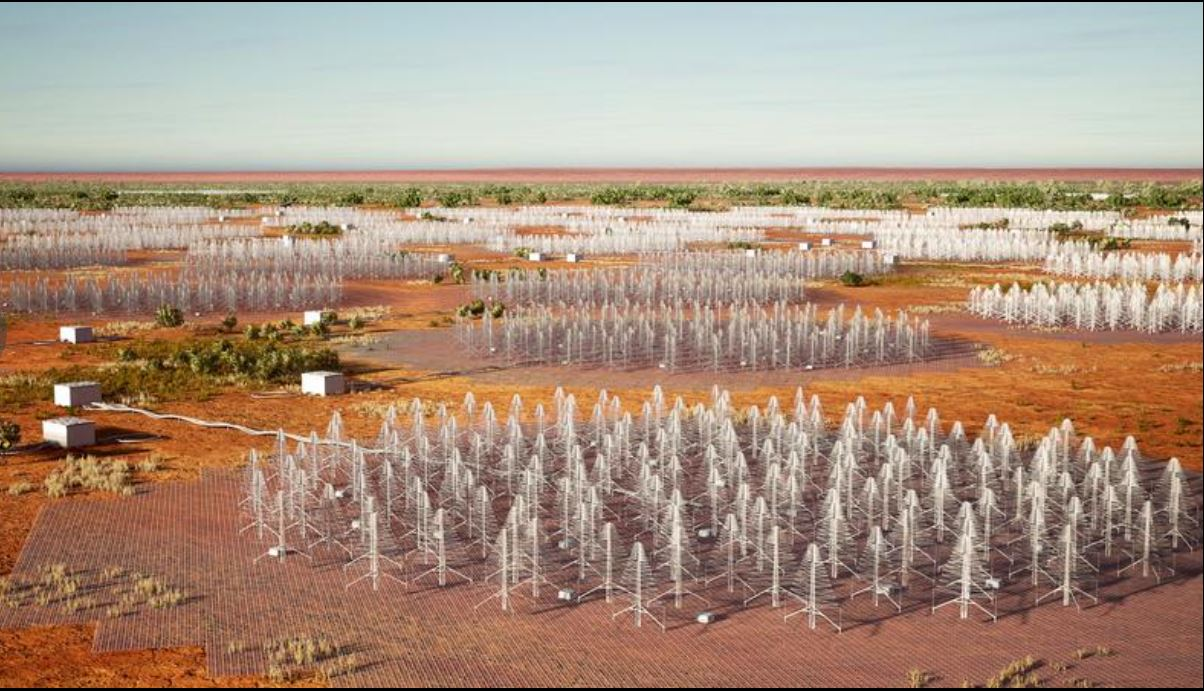
\includegraphics[width=1.10\linewidth,height=3.00cm]{assets/SKA Image.jpeg}};
\end{tikzpicture}
\end{center}

\onslide<2->
\vspace{0.80em}
{
\setbeamercolor{block title}{fg=white,bg=blue!70!black}
\setbeamercolor{block body}{bg=blue!8}
\bayesgridblock[2.05cm]{Statistical Inference}{%
$\triangleright$ Traditional sampling: many likelihood evaluations\\[0.2em]
$\triangleright$ SBI: many simulated datasets\\[0.2em]
$\triangleright$ \textbf{Inference cost grows rapidly}
}
}
\end{column}
\end{columns}
\end{frame}

\begin{frame}{Radio Astronomy $\leftrightarrow$ Accelerators}
\vspace{-0.6em}
\begin{columns}[T,totalwidth=\textwidth]
\begin{column}{0.48\textwidth}
\onslide<1->
{
\setbeamercolor{block title}{fg=white,bg=blue!70!black}
\setbeamercolor{block body}{bg=blue!8}
\bayesgridblock[4.70cm]{Radio Astronomy}{%
\(\triangleright\) Bulk linear algebra operations:\\[0.25em]
\vspace{0.80em}
{\raggedright
\hspace{0.50em} \(\circ\) Matrix multplications\\[0.15em]
\hspace{0.50em} \(\circ\) Fourier transforms\\[0.15em]
\hspace{0.50em} \(\circ\) Matrix inversions\par}
\vspace{1.00em}
\(\triangleright\) Intrinsic batch dimensions:\\[0.35em]
\vspace{0.80em}
{\centering
\(
\begin{array}{@{}l@{\hspace{0.8em}}l@{}}
\hspace{0.50em} \circ\ \text{Baselines}\ (b) & \circ\ \text{Frequency}\ (\nu)\\[0.15em]
\hspace{0.50em} \circ\ \text{Time}\ (t) & \circ\ \text{Polarisation}\ (p)
\end{array}
\)\par}
}
}
\end{column}
\begin{column}{0.48\textwidth}
\onslide<2->
{
\setbeamercolor{block title}{fg=white,bg=teal!75!black}
\setbeamercolor{block body}{bg=teal!10}
\bayesgridblock[2.10cm]{LLM-era Accelerators}{%
\(\triangleright\) Transformer architectures:\\[0.12em]
{\raggedright\footnotesize
\hspace{0.50em} \(\circ\) Dense matrix multiplication\\[0.10em]
\hspace{0.50em} \(\circ\) Specialised tensor cores\par}
\vspace{0.12em}
\(\triangleright\) High-bandwidth memory\\[0.18em]
\(\triangleright\) Native multi-device scaling
}
}

\onslide<3->
\vspace{0.05em}
{
\setbeamercolor{block title}{fg=white,bg=CambridgeDark}
\setbeamercolor{block body}{fg=CambridgeDark,bg=CambridgeCore!20!normal text.bg}
\bayesgridblock[1.70cm]{Accelerator Software}{%
\(\triangleright\) High-level array programming, low-level kernel execution\\[0.18em]
\(\triangleright\) Accelerator-level compilation without writing CUDA\\[0.18em]

}
}
\end{column}
\end{columns}

\onslide<4->
\vspace{-0.01em}
{
\setbeamercolor{block title}{fg=white,bg=red!75!black}
\setbeamercolor{block body}{bg=red!10}
\begin{beamerboxesrounded}[upper=block title,lower=block body,shadow=true,width=\textwidth]{\textbf{Takeaway}}
\small
\(\triangleright\) Radio-astronomy inference maps naturally to LLM-era compute\\[0.15em]
\(\triangleright\) Redefining the scale and complexity with which we can perform inference
\end{beamerboxesrounded}
}
\end{frame}

\begin{frame}{Next-Generation AI Supercomputers}
\scriptsize
\begin{columns}[T,totalwidth=\textwidth]
\begin{column}{0.52\textwidth}
\vspace{-0.5em}
{
\setbeamercolor{block title}{fg=white,bg=blue!70!black}
\setbeamercolor{block body}{bg=blue!8}
\bayesgridblock[0.8cm]{Isambard-AI}{%
\textbullet\ 1,320 nodes overall\\[0.18em]
\textbullet\ 5,280 GH200 superchips
}
}
\vspace{0.35em}
{
\setbeamercolor{block title}{fg=white,bg=teal!75!black}
\setbeamercolor{block body}{bg=teal!10}
\bayesgridblock[2.8cm]{GH200 Node}{%
\textbullet\ 4x Grace ARM CPUs\\[0.18em]
\hspace{1.2em}\textbullet\ 288 CPU cores\\[0.18em]
\hspace{1.2em}\textbullet\ 512 GB CPU memory\\[0.18em]
\textbullet\ 4x Hopper GPUs\\[0.18em]
\hspace{1.2em}\textbullet\ 384 GB high-bandwidth memory\\[0.18em]
\textbullet\ 896 GB total memory
}
}
\vspace{0.35em}
{
\setbeamercolor{block title}{fg=white,bg=red!75!black}
\setbeamercolor{block body}{bg=red!10}
\bayesgridblock[0.8cm]{Future Directions}{%
\textbullet\ Google TPUs\\[0.18em]
\textbullet\ Promising for SKA-scale inference
}
}
\end{column}
\begin{column}{0.48\textwidth}
\begin{flushright}
\begin{minipage}{0.86\linewidth}
\centering
\makebox[\linewidth][c]{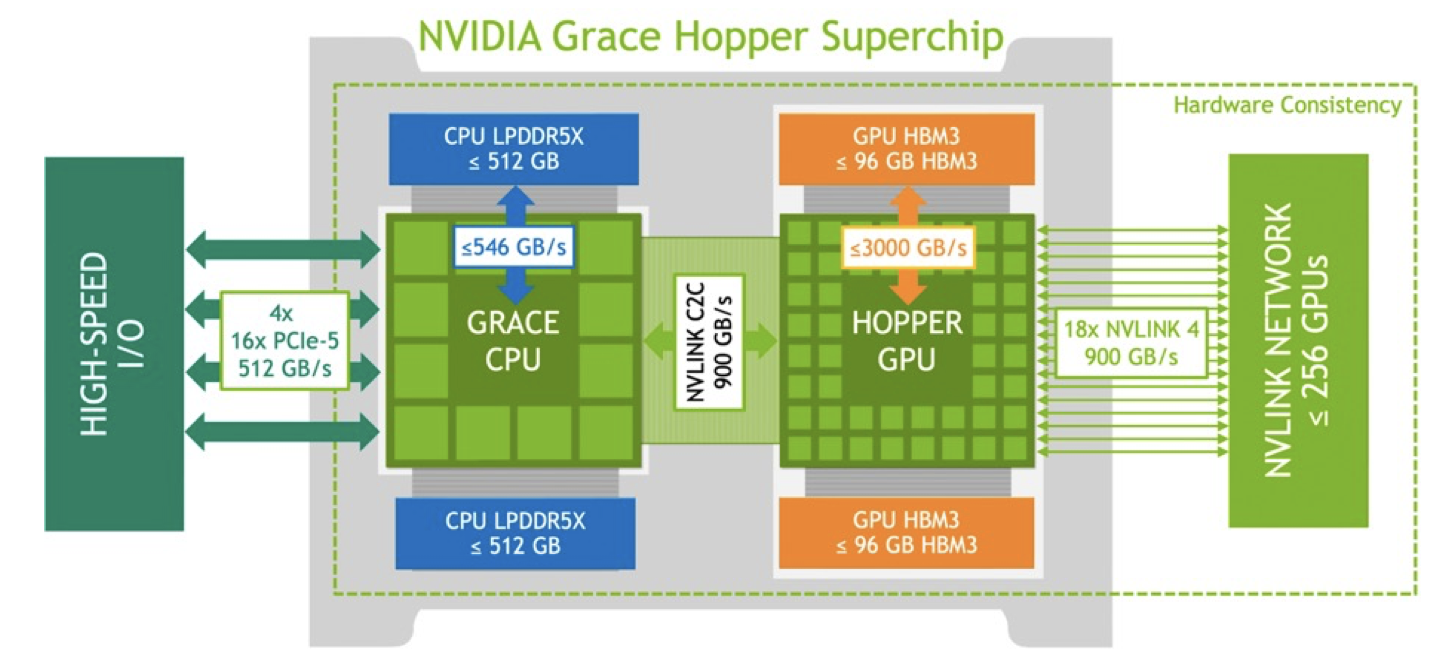
\includegraphics[height=2.50cm]{assets/GH_Chip.png}}

\vspace{2.0em}
\makebox[\linewidth][c]{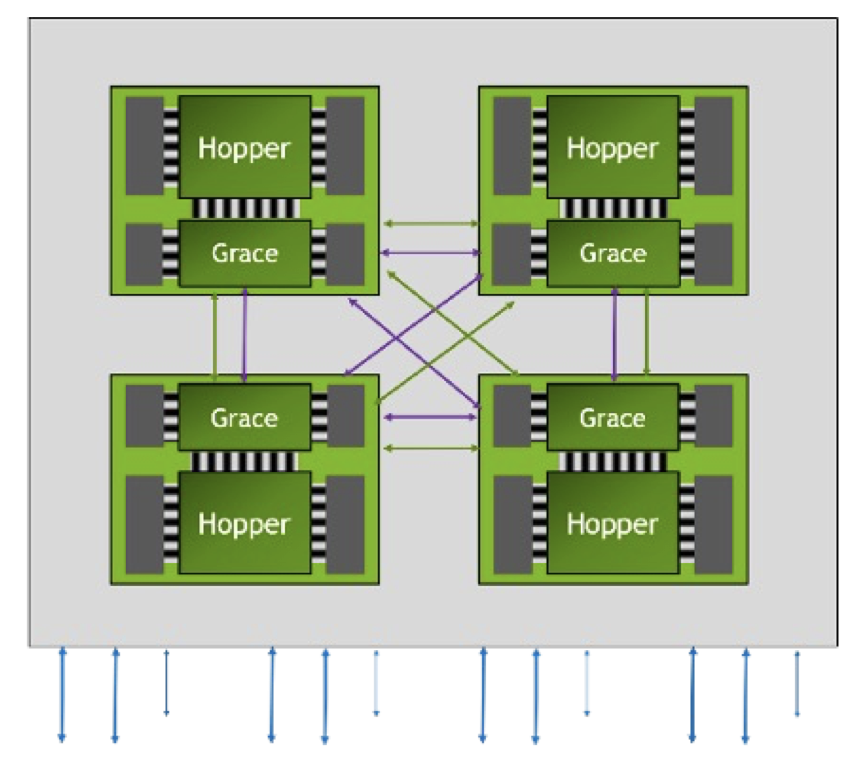
\includegraphics[height=2.95cm,trim=0 0.55cm 0 0,clip]{assets/4GPUNODE.png}}
\end{minipage}
\end{flushright}
\vfill
\raggedleft
\tiny Source: \href{https://developer.nvidia.com/blog/nvidia-grace-hopper-superchip-architecture-in-depth/}{NVIDIA Grace Hopper Superchip Architecture}
\end{column}
\end{columns}
\end{frame}


\begin{frame}{An Introduction to JAX}
\footnotesize
\begin{columns}[T,totalwidth=\textwidth]
\begin{column}{0.28\textwidth}
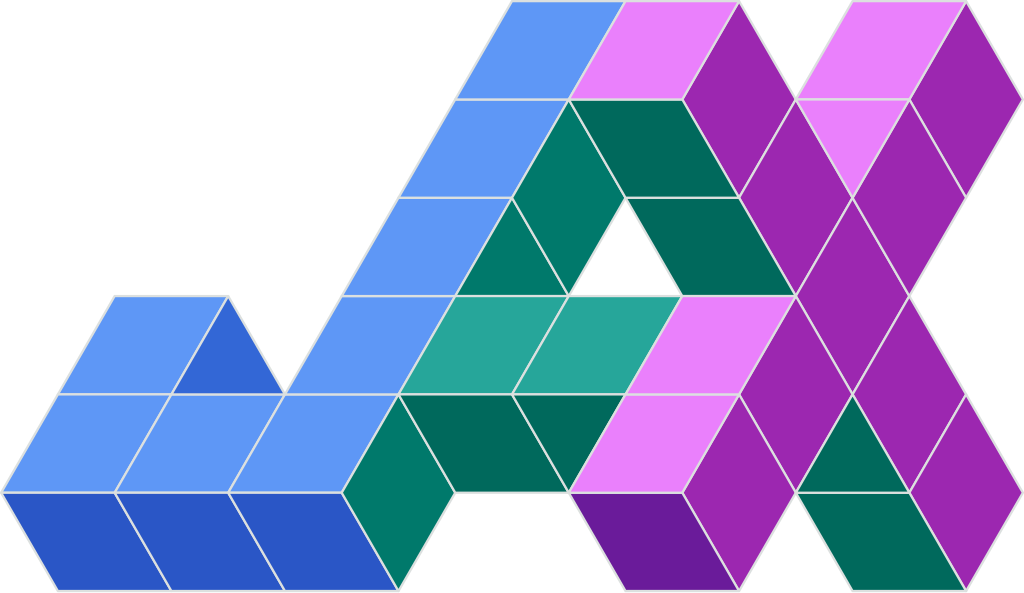
\includegraphics[width=0.75\linewidth]{assets/jax.png}

\vspace{0.2em}
\footnotesize
\textbf{High-performance numerical-computing}\\
\textbf{and large-scale machine learning}

\vspace{0.7em}
\hspace{-0.35em}
\scriptsize
\begin{tabular}{@{}c@{}}
High-level array code\\[-0.05em]
\(\Downarrow\)\\[-0.05em]
JAX tracing\\[-0.05em]
\(\Downarrow\)\\[-0.05em]
XLA compilation\\[-0.05em]
\(\Downarrow\)\\[-0.05em]
Hardware-optimised\\
kernels\\[-0.05em]
\(\Downarrow\)\\[-0.05em]
CPU / GPU / TPU\\
execution
\end{tabular}
\end{column}
\pause
\begin{column}{0.715\textwidth}
\vspace{-0.05em}
\begin{beamerboxesrounded}[upper=block title,lower=block body,shadow=true,width=\linewidth]{\textbf{XLA Compilation}}
\small
\scriptsize
\begin{itemize}
    \item Compiles high-level array code into optimised machine code
    \item Combines Python productivity with compiled-performance execution
\end{itemize}
\vspace{-1.35em}
\[
f(x) \quad\Longrightarrow\quad \texttt{jax.jit}(f)(x)
\]
\end{beamerboxesrounded}
\pause 
\vspace{0.2em}
\vfill
\begin{beamerboxesrounded}[upper=block title,lower=block body,shadow=true,width=\linewidth]{\textbf{Parallelisation/ Distribution}}
\small
\scriptsize
\begin{itemize}
    \item \textbf{Vectorisation}: automatic parallelisation over batches of data
    \item \textbf{Sharding}: distributing arrays and workloads across \\ \hspace{1.3cm} multi-GPU / multi-TPU architectures
\end{itemize}
\end{beamerboxesrounded}
\pause 

\vspace{0.2em}
\vfill
\begin{beamerboxesrounded}[upper=block title,lower=block body,shadow=true,width=\linewidth]{\textbf{Automatic Differentiation}}
\small
\vspace{-0.25em}
\[
(\nabla f)(x)_i = \frac{\partial f}{\partial x_i}(x)
\quad\Longrightarrow\quad 
\texttt{jax.grad(f)(x)}
\]
\scriptsize \faGithub\ \href{https://github.com/JacobTutt/dual_autodiff_package}{JacobTutt/dual\_autodiff\_package}
\end{beamerboxesrounded}
\end{column}
\end{columns}
\end{frame}

\begin{frame}{JAX Ecosystem}
\small
\begin{columns}[T,totalwidth=\textwidth]
\begin{column}{0.32\textwidth}
\begin{center}
\begin{minipage}[t][2.6cm][c]{\linewidth}
\centering
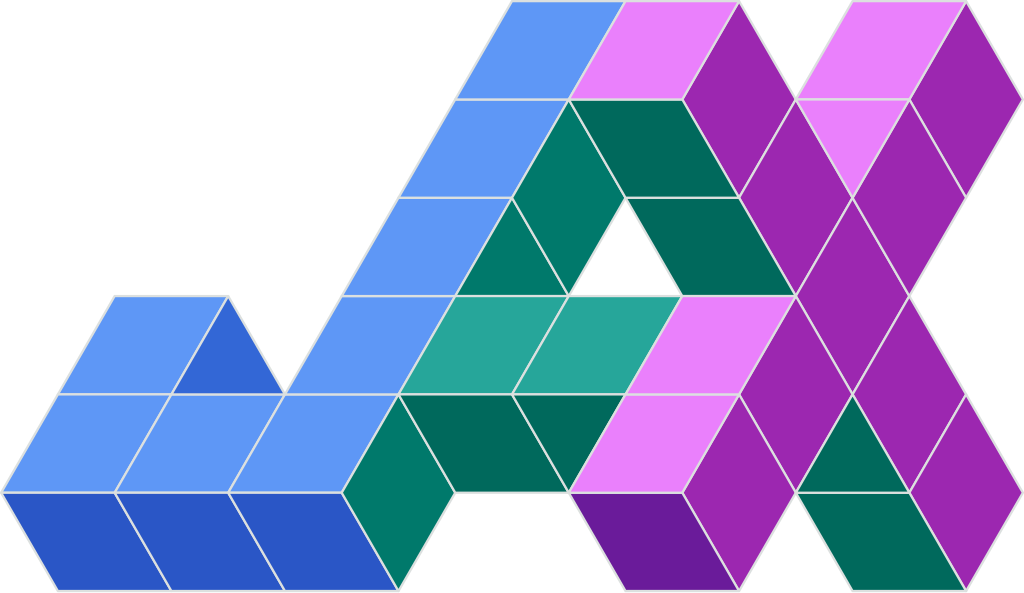
\includegraphics[height=1.65cm]{assets/jax.png}\\[0.3em]
\textbf{JAX}
\end{minipage}
\end{center}
\end{column}
\begin{column}{0.32\textwidth}
\begin{center}
\begin{minipage}[t][2.6cm][c]{\linewidth}
\centering

\includegraphics[height=1.9cm]{assets/optax.png}\\[0.3em]
\textbf{Optax}
\end{minipage}
\end{center}
\end{column}
\begin{column}{0.32\textwidth}
\begin{center}
\begin{minipage}[t][2.6cm][c]{\linewidth}
\centering

\includegraphics[height=1.9cm]{assets/blackjax.jpeg}\\[0.3em]
\textbf{BlackJAX}
\end{minipage}
\end{center}
\end{column}
\end{columns}

\vspace{0.6em}
\begin{columns}[T,totalwidth=\textwidth]
\begin{column}{0.32\textwidth}
\begin{center}
\begin{minipage}[t][2.6cm][c]{\linewidth}
\centering

\includegraphics[height=1.9cm]{assets/flax_logo.png}\\[0.3em]
\textbf{Flax}
\end{minipage}
\end{center}
\end{column}
\begin{column}{0.32\textwidth}
\begin{center}
\begin{minipage}[t][2.6cm][c]{\linewidth}
\centering

\includegraphics[height=2.15cm]{assets/xla.png}\\[0.3em]
\textbf{XLA}
\end{minipage}
\end{center}
\end{column}
\begin{column}{0.32\textwidth}
\begin{center}
\begin{minipage}[t][2.6cm][c]{\linewidth}
\centering

\includegraphics[height=1.9cm]{assets/jaxtronomy_logo.png}\\[0.3em]
\href{https://github.com/JAXtronomy/awesome-JAXtronomy}{\textbf{JAXtronomy}}
\end{minipage}
\end{center}
\end{column}
\end{columns}
\end{frame}

\begin{frame}{Case Study I: Global 21-cm Cosmology}
\begin{center}
\begin{tikzpicture}
  \node[inner sep=0] (pipeline) {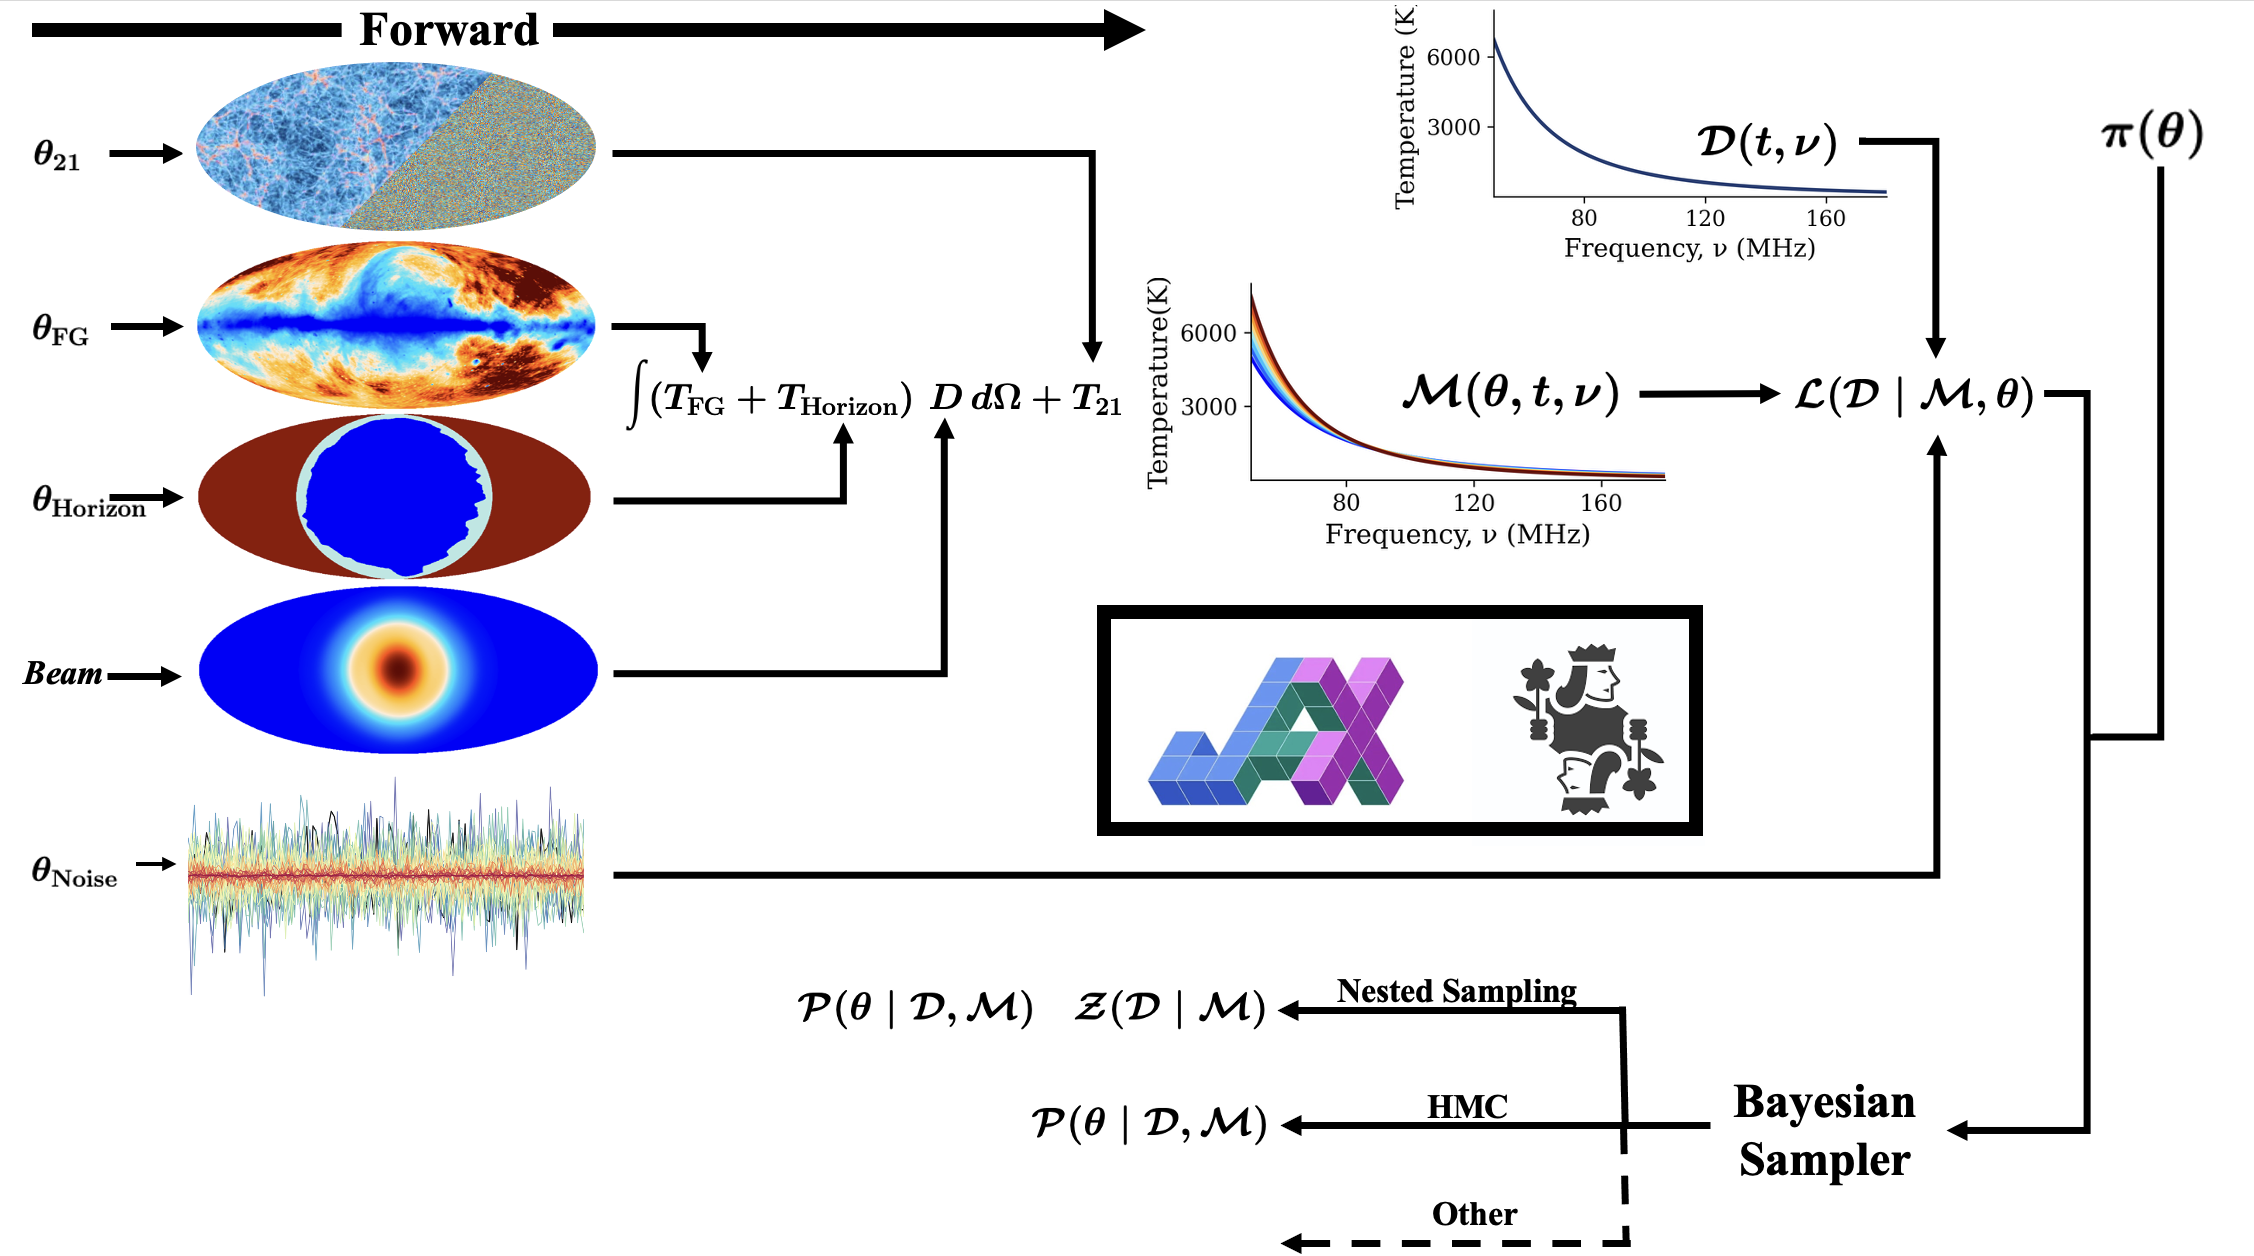
\includegraphics[width=0.96\linewidth]{assets/REACH_Pipeline.png}};
  \node[anchor=south west,inner sep=0] at ([xshift=0.12cm,yshift=-0.18cm]pipeline.south west)
    {
\includegraphics[height=1.20cm]{../../theme/high-res.png}};
\end{tikzpicture}
\end{center}
\vspace{-0.35em}
\noindent
\makebox[0pt][l]{\tiny with P. Sims, J. Pattison, D. Anstey, S. Leeney and E. de Lera Acedo}%
\hfill
{\tiny Source: \href{https://arxiv.org/abs/2603.13196}{arXiv:2603.13196}}\par
\end{frame}

\begin{frame}{REACH: Scaling Behaviour}
\begin{columns}[T,totalwidth=\textwidth]
\begin{column}{0.49\textwidth}
\scriptsize \textbf{Model Complexity}

\vspace{0.2em}
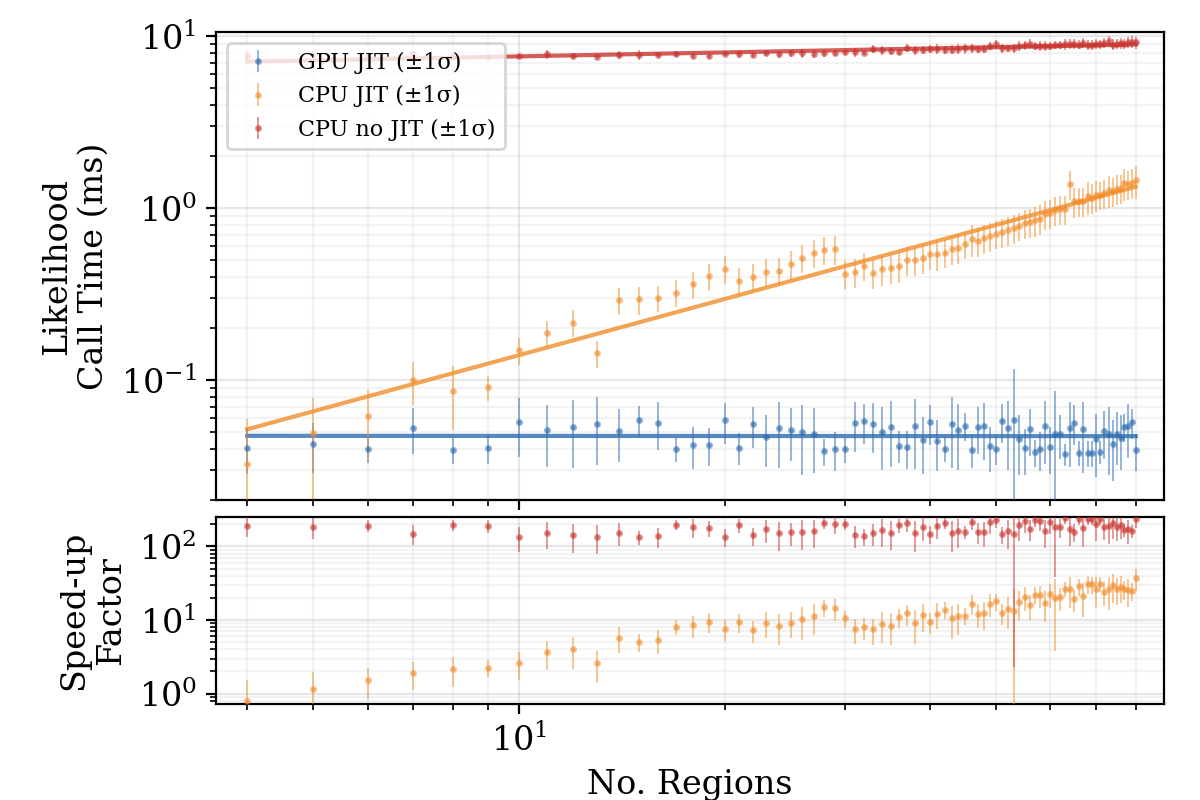
\includegraphics[width=\linewidth]{assets/likelihood_timing_plot_loglog.png}
\end{column}
\begin{column}{0.49\textwidth}
\scriptsize \textbf{Data Volume}

\vspace{0.2em}
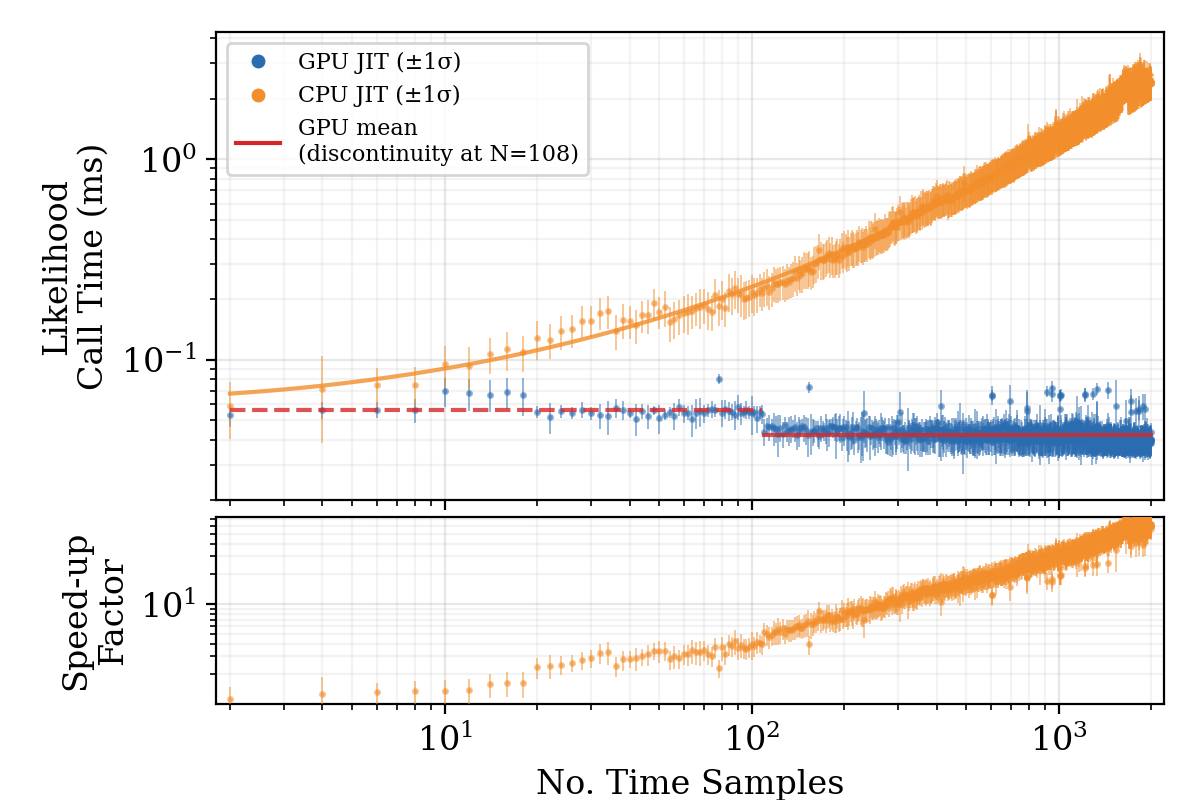
\includegraphics[width=\linewidth]{assets/likelihood_timing_plot_ntimes_loglog.png}
\end{column}
\end{columns}

\vspace{0.15em}
\noindent\hfill
{\tiny *GPU: NVIDIA A100 (40GB) \qquad *CPU: Intel Cascade Lake CPU}\par

\vspace{0.20em}
\bayesgridblock[1.10cm]{What this means for REACH:}{%
\scriptsize
\begin{itemize}
    \item Full first-year early dataset fits: \(\sim\)4000 spectra at near single-spectrum cost
    \item More complex foreground models for higher-resolution low-frequency sky maps
\end{itemize}
}
\noindent
\vspace{-0.25em}
\makebox[0pt][l]{\tiny with P. Sims, J. Pattison, D. Anstey, S. Leeney and E. de Lera Acedo}%
\hfill
{\tiny Source: \href{https://arxiv.org/abs/2603.13196}{arXiv:2603.13196}}\par
\end{frame}

\begin{frame}{BaNTER Validation Framework}
\footnotesize
\begin{columns}[T,totalwidth=\textwidth]
\begin{column}{0.48\textwidth}
\bayesgridblock[2.25cm]{Motivation}{%
\scriptsize $\triangleright$ Two hypothesised models \(M_\mathrm{FG}\)/\(M_\mathrm{FG+21}\):
\[
\ln B_{\mathrm{det}}
=
\ln\!\left(
\frac{\mathcal{Z}_{\mathrm{FG+21}}}{\mathcal{Z}_{\mathrm{FG}}}
\right)
\]
\scriptsize $\triangleright$ A high detection Bayes factor alone is not enough\\[0.18em]
}
\vspace{0.2em}
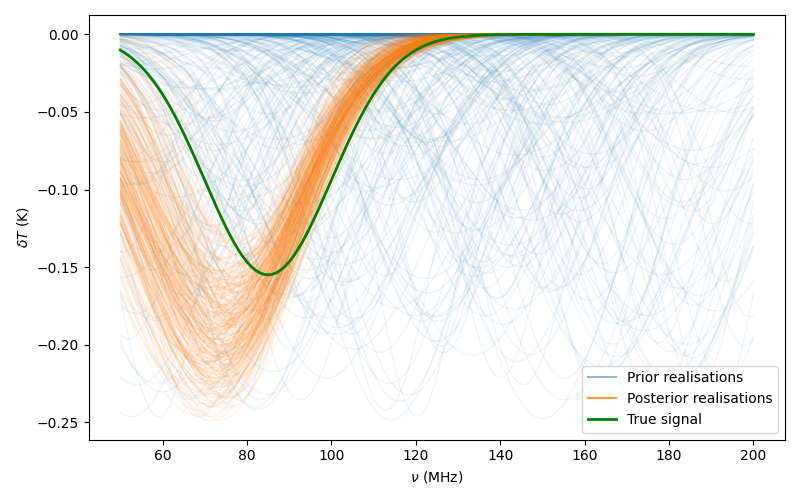
\includegraphics[width=\linewidth]{assets/signal_comparison.png}
\end{column}

\begin{column}{0.48\textwidth}
\onslide<2->{
{
\setbeamercolor{block title}{fg=white,bg=blue!70!black}
\setbeamercolor{block body}{bg=blue!8}
\bayesgridblock[1.80cm]{Metric 1: Null Test}{%
\[
\ln B_{\mathrm{val}}
=
\ln\!\left(
\frac{\mathcal{Z}_{\mathrm{FG+21}}^{\mathrm{v}}}
{\mathcal{Z}_{\mathrm{FG}}^{\mathrm{v}}}
\right)
\]
\scriptsize Fit signal-free validation data\par
\scriptsize \(\triangleright\) Fail if \(\ln B_{\mathrm{val}} \ge 0\)\par
}
}
}

\onslide<3->{
\vspace{0.25em}
{
\setbeamercolor{block title}{fg=white,bg=red!75!black}
\setbeamercolor{block body}{bg=red!10}
\bayesgridblock[1.45cm]{Metric 2: Residual Structure}{%
\[
q_i = \mathbb{P}\!\left( \mathcal{L}_{\mathrm{noise}} \le \overline{\mathcal{L}}_i \right)
\]
\scriptsize Ask whether the residuals are noise-like\par
\scriptsize \(\triangleright\) Require \(q_i \ge q_{\mathrm{threshold}}\)\par
}
}
}
\onslide<4->{
\vspace{0.25em}
{
\setbeamercolor{block title}{fg=white,bg=teal!75!black}
\setbeamercolor{block body}{bg=teal!10}
\bayesgridblock[0.6cm]{Evidence Evaluation}{%
\scriptsize BlackJAX Nested Slice Sampling\par
\scriptsize \faGithub\ \href{https://github.com/handley-lab/blackjax}{BlackjaxNSS}\par
}
}
}
\end{column}
\end{columns}
\vfill
\vspace{-0.4em}
\hfill{\tiny \href{https://github.com/uksrc/ValSKA-HERA-beam-FWHM}{UKSRC Validation Team}}\par
\vspace{-0.2em}
\noindent
\makebox[0pt][l]{\tiny with P. Sims, J. Pattison, D. Anstey, S. Leeney and E. de Lera Acedo}%
\hfill
{\tiny Sources: \href{https://arxiv.org/abs/2603.13196}{arXiv:2603.13196}; \href{https://arxiv.org/abs/2502.14029}{arXiv:2502.14029}}\par
\end{frame}

\begin{frame}{Validation Across Model Configurations}
\begin{center}

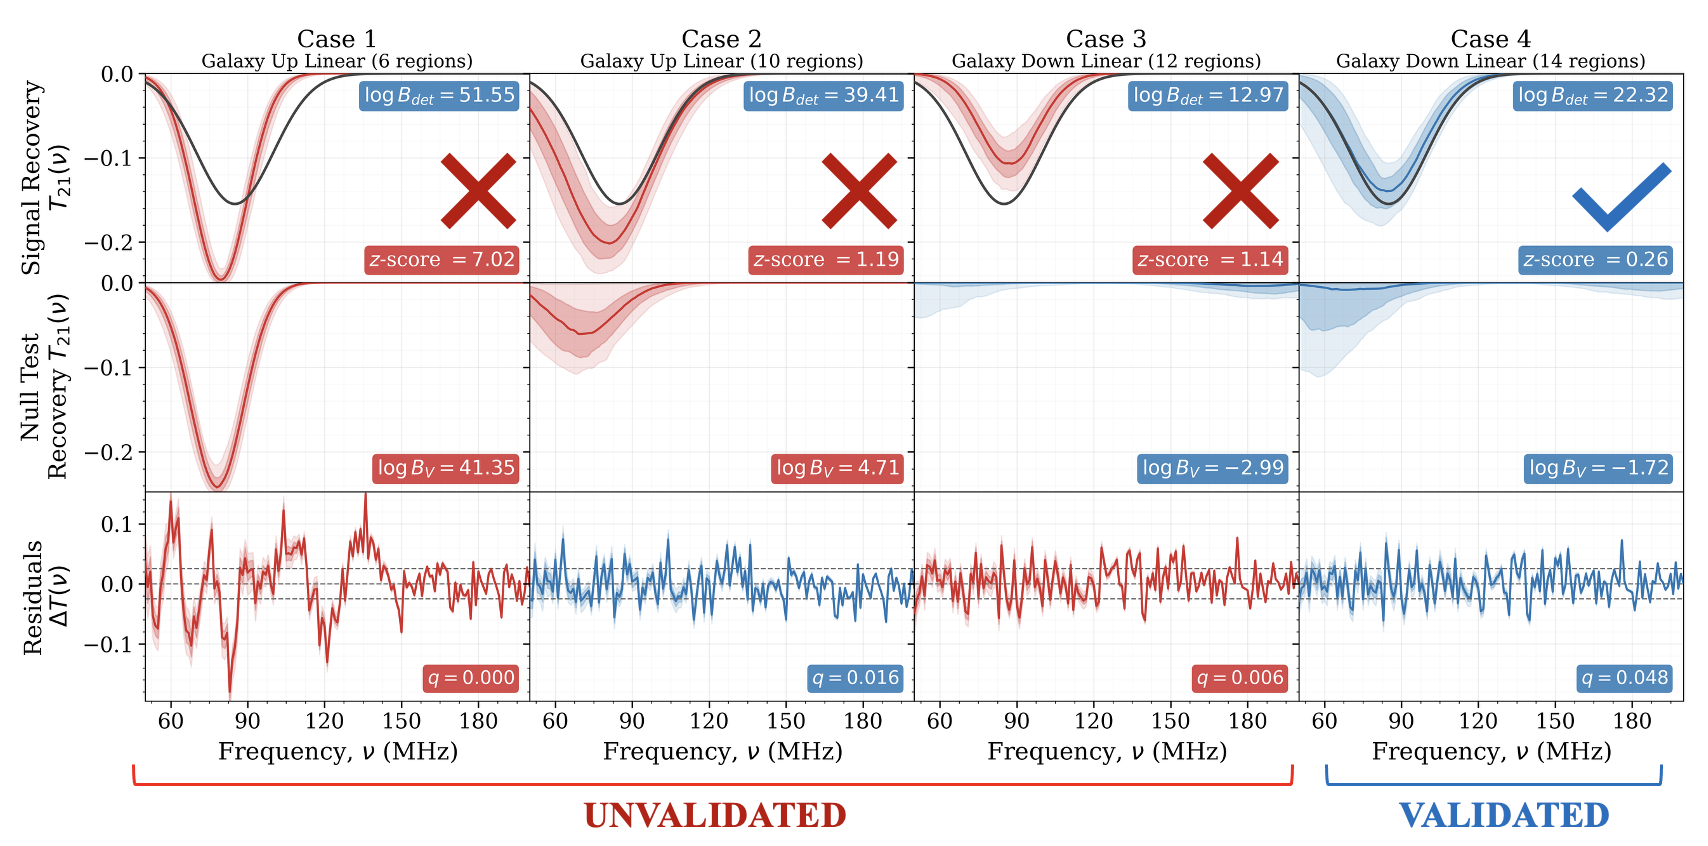
\includegraphics[width=0.83\linewidth]{assets/validation_grid.png}
\end{center}
\vspace{-0.5em}
\bayesgridblock[1.2cm]{Key Takeaways}{%
\vspace{-0.2em}
\scriptsize
\begin{itemize}\setlength{\itemsep}{0.1em}
    \item Validated recovery rejects cases that \(\ln B_{\mathrm{det}}\) alone would accept
    \item 1052 nested-sampling runs: \\
    \hspace{0.15cm}$\triangleright$ \(\sim 100\) CPU years \(\rightarrow\) under 2 GPU days (\(\sim 100\times\) lower cost)
\end{itemize}
}
\vspace{-0.6em}
\noindent
\makebox[0pt][l]{\tiny with P. Sims, J. Pattison, D. Anstey, S. Leeney and E. de Lera Acedo}%
\hfill
{\tiny Sources: \href{https://arxiv.org/abs/2603.13196}{arXiv:2603.13196}; \href{https://arxiv.org/abs/2502.14029}{arXiv:2502.14029}}\par
\end{frame}

\begin{frame}{Opening the Door to SBI}
\begin{columns}[T,totalwidth=\textwidth]
\begin{column}{0.43\textwidth}
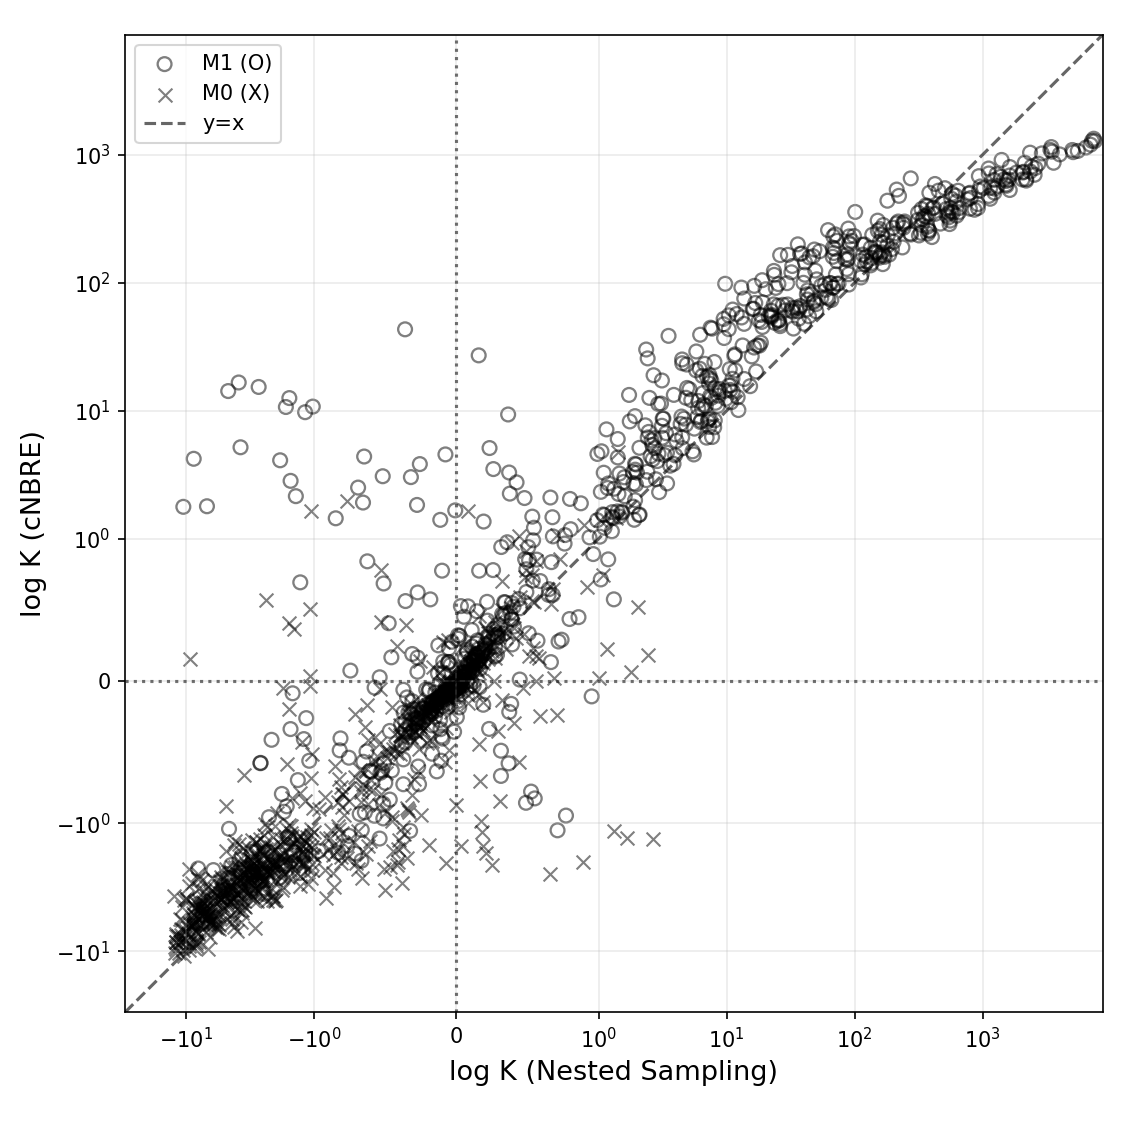
\includegraphics[width=0.98\linewidth]{assets/cnbre_ns_scatter.png}
\end{column}
\begin{column}{0.55\textwidth}
\scriptsize

\vspace{0.25em}
{
\setbeamercolor{block title}{fg=white,bg=red!75!black}
\setbeamercolor{block body}{bg=red!10}
\bayesgridblock[3.20cm]{Conditional Bayes Neural Ratio Estimation}{%
$\triangleright$ \textbf{Sub-ms forward model}\\[0.10em]
$\triangleright$ \textbf{What this enables for SBI}\\[0.10em]
\hspace*{0.8em}\(\circ\) Dynamic simulations during training\\[0.10em]
\hspace*{0.8em}\(\circ\) End-to-end gradients\\[0.10em]
\hspace*{0.8em}\(\circ\) No fixed simulation set:\\[0.10em]
\hspace*{0.8em} \(\Rightarrow\) Better coverage of the prior\\[0.10em]
\hspace*{0.8em} \(\Rightarrow\) Less overfitting
}
}
\end{column}
\end{columns}

\vspace{3em}
\noindent
\makebox[0pt][l]{\tiny with \textbf{S. Leeney}, T. Gessey-Jones, W. Handley, E. de Lera Acedo, H. Bevins}%
\hfill
{\tiny Source: Leeney et al. (in Prep)}\par
\vspace{-2em}
\end{frame}

\begin{frame}{Case Study II: BayesEoR}
\begin{minipage}{0.50\textwidth}
\bayesgridblock[0.7cm]{BayesEoR Approach}{%
{\scriptsize
$\triangleright$ Foreground Reconstruction\\[0.08em]
$\triangleright$ 21-cm Power Spectrum Analysis
}}
\end{minipage}

\vspace{0.15em}
{\centering
\resizebox{0.92\textwidth}{!}{%
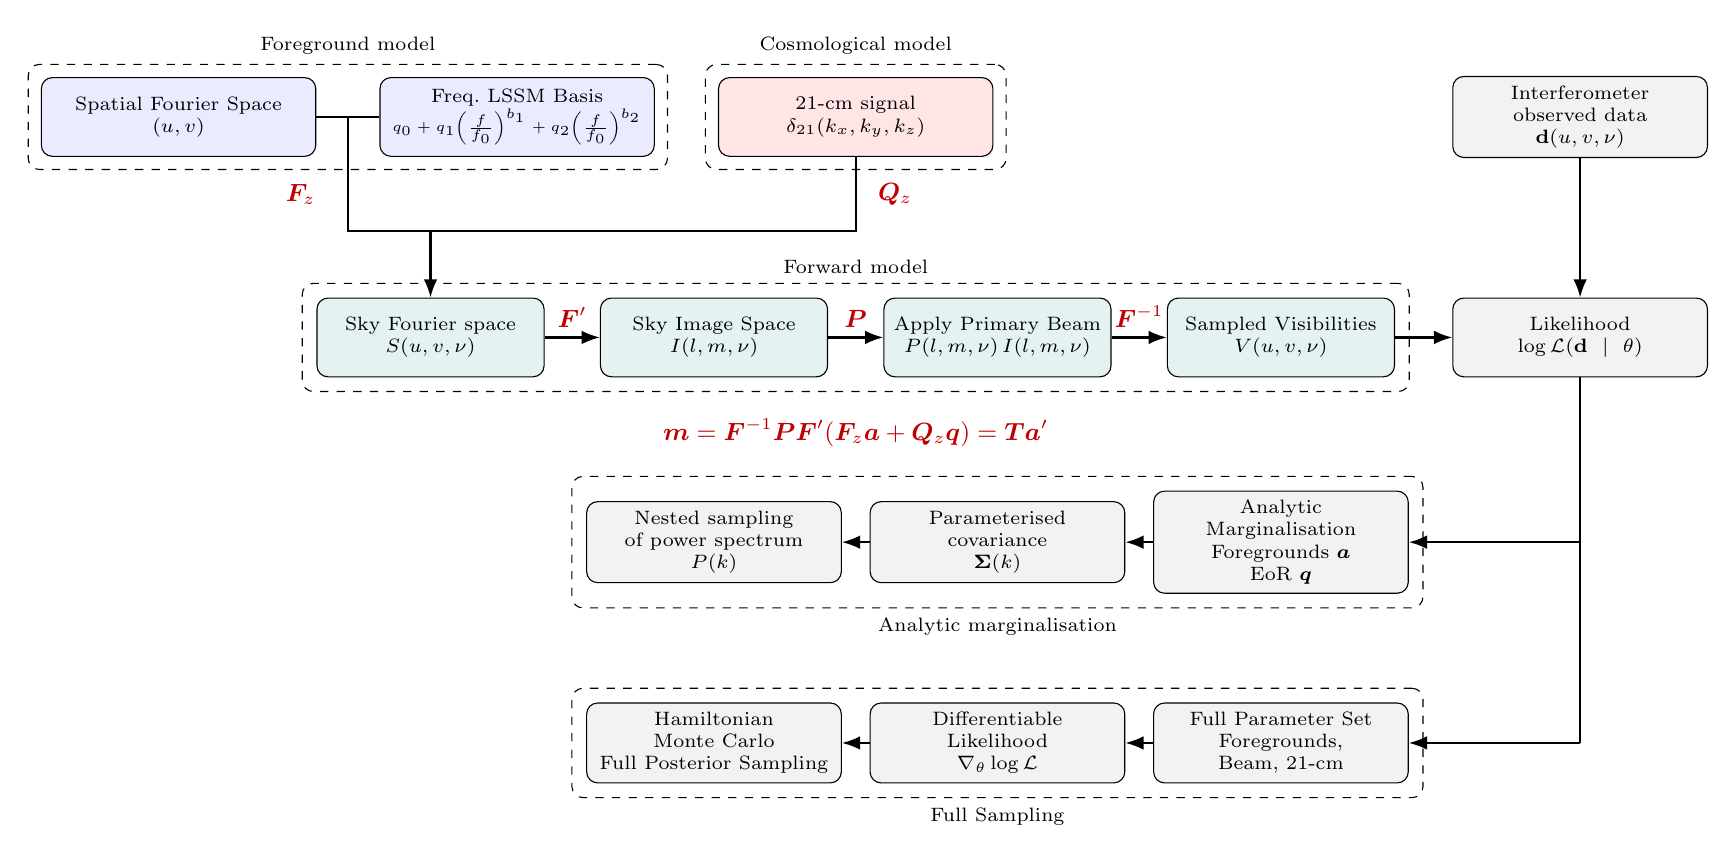
\begin{tikzpicture}[
    every node/.style={font=\scriptsize},
    flow/.style={-Latex, thick},
    fgbox/.style={draw, rounded corners, align=center, minimum height=1.0cm, text width=2.45cm, fill=blue!8},
    signalbox/.style={draw, rounded corners, align=center, minimum height=1.0cm, text width=2.45cm, fill=red!10},
    opbox/.style={draw, rounded corners, align=center, minimum height=1.0cm, text width=2.65cm, fill=teal!10},
    likebox/.style={draw, rounded corners, align=center, minimum height=1.0cm, text width=3cm, fill=gray!10}
]
\node[fgbox,text width=3.25cm] (fguv) at (0.0,3.0) {Spatial Fourier Space\\$(u,v)$};
\node[fgbox,text width=3.25cm] (lssm) at (4.3,3.0) {Freq.\ LSSM Basis\\{\tiny $q_0 + q_1\!\left(\frac{f}{f_0}\right)^{b_1} + q_2\!\left(\frac{f}{f_0}\right)^{b_2}$}};
\node[signalbox,text width=3.25cm] (kspace) at (8.6,3.0) {21-cm signal\\$\delta_{21}(k_x,k_y,k_z)$};
\node[likebox] (data) at (17.8,3.0) {Interferometer\\observed data\\$\mathbf{d}(u,v,\nu)$};

\node[opbox] (uvsky) at (3.2,0.2) {Sky Fourier space\\$S(u,v,\nu)$};
\node[opbox] (sky) at (6.8,0.2) {Sky Image Space\\$I(l,m,\nu)$};
\node[opbox] (beam) at (10.4,0.2) {Apply Primary Beam\\$P(l,m,\nu)\,I(l,m,\nu)$};
\node[opbox] (vis) at (14.0,0.2) {Sampled Visibilities\\$V(u,v,\nu)$};
\node[likebox] (like) at (17.8,0.2) {Likelihood\\$\log \mathcal{L}(\mathbf{d}\mid\theta)$};

\node[likebox] (compress) at (14.0,-2.4) {Analytic Marginalisation\\Foregrounds $\bm{a}$\\EoR $\bm{q}$};
\node[likebox] (sigma) at (10.4,-2.4) {Parameterised covariance\\$\bm{\Sigma}(k)$};
\node[likebox] (sample) at (6.8,-2.4) {Nested sampling of power spectrum\\ $P(k)$};
\node[likebox] (fullparams) at (14.0,-4.95) {Full Parameter Set\\Foregrounds, Beam, 21-cm};
\node[likebox] (gradlike) at (10.4,-4.95) {Differentiable Likelihood\\$\nabla_{\theta}\log \mathcal{L}$};
\node[likebox] (hmc) at (6.8,-4.95) {Hamiltonian Monte Carlo\\Full Posterior Sampling};

\coordinate (fgmid) at (2.15,3.0);
\coordinate (merge) at (3.2,1.55);
\coordinate (kjoin) at (8.6,1.55);
\draw[thick] (fgmid) -- ++(0,-1.45) -| (merge);
\draw[thick] (fguv.east) -- (lssm.west);
\draw[thick] (kspace.south) -- (kjoin) -- (merge);
\node[font=\small] at (1.55,2.02) {\textcolor{red!75!black}{\(\bm{F}_{z}\)}};
\node[font=\small] at (9.10,2.02) {\textcolor{red!75!black}{\(\bm{Q}_{z}\)}};
\draw[flow] (merge) -- (uvsky.north);
\draw[flow] (uvsky) -- node[midway, above, font=\small] {\textcolor{red!75!black}{\(\bm{F}'\)}} (sky);
\draw[flow] (sky) -- node[midway, above, font=\small] {\textcolor{red!75!black}{\(\bm{P}\)}} (beam);
\draw[flow] (beam) -- node[midway, above, font=\small] {\textcolor{red!75!black}{\(\bm{F}^{-1}\)}} (vis);
\draw[flow] (vis) -- (like);
\draw[flow] (data.south) -- (like.north);

\coordinate (branchanalytic) at (like.south |- compress.east);
\coordinate (branchfull) at (like.south |- fullparams.east);
\draw[thick] (like.south) -- (branchfull);
\draw[flow] (branchanalytic) -- (compress.east);
\draw[flow] (branchfull) -- (fullparams.east);
\draw[flow] (compress) -- (sigma);
\draw[flow] (sigma) -- (sample);
\draw[flow] (fullparams) -- (gradlike);
\draw[flow] (gradlike) -- (hmc);

\node[draw, dashed, rounded corners, fit=(fguv)(lssm), inner sep=0.16cm, label={[font=\scriptsize]above:Foreground model}] {};
\node[draw, dashed, rounded corners, fit=(kspace), inner sep=0.16cm, label={[font=\scriptsize]above:Cosmological model}] {};
\node[draw, dashed, rounded corners, fit=(uvsky)(sky)(beam)(vis), inner sep=0.18cm, label={[font=\scriptsize]above:Forward model}] (forwardfit) {};
\node[font=\small, below=0.22cm of forwardfit.south] {\textcolor{red!75!black}{\(\bm{m} = \bm{F}^{-1}\bm{P}\bm{F}'(\bm{F}_{z}\bm{a} + \bm{Q}_{z}\bm{q}) = \bm{T}\bm{a}'\)}};
\node[draw, dashed, rounded corners, fit=(compress)(sigma)(sample), inner sep=0.18cm, label={[font=\scriptsize]below:Analytic marginalisation}] {};
\node[draw, dashed, rounded corners, fit=(fullparams)(gradlike)(hmc), inner sep=0.18cm, label={[font=\scriptsize]below:Full Sampling}] {};
\end{tikzpicture}
}\par}
\vfill
{\raggedright\tiny with P. Sims, D. Anstey and E. de Lera Acedo\par}
\end{frame}




\begin{frame}{Takeaways}
\small
\uncover<1->{%
\bayesgridblock[1.55cm]{Hardware}{%
Radio-astronomy inference workloads map naturally onto accelerator systems developed for AI: massively parallel, tensor-core, multi-device hardware.
}
}

\vspace{0.45em}
\uncover<2->{%
{
\setbeamercolor{block title}{fg=white,bg=blue!70!black}
\setbeamercolor{block body}{bg=blue!8}
\bayesgridblock[1.35cm]{Software}{%
Modern software libraries, such as JAX, significantly reduce the barrier to using these architectures effectively.
}
}
}

\vspace{0.45em}
\uncover<3->{%
{
\setbeamercolor{block title}{fg=white,bg=red!70!black}
\setbeamercolor{block body}{bg=red!8}
\bayesgridblock[1.15cm]{Impact}{%
Acceleration of the REACH and BayesEoR Pipelines illustrate how these methods are changing the speed, scale, complexity and rigor of radio-astronomy inference.
}
}
}
\end{frame}

\begin{frame}{Questions}
\centering
\vspace{1em}
\textbf{Thank you for your attention!}
\vspace{1.5em}
\begin{minipage}{0.8\textwidth}
\centering
\footnotesize
\vspace{0.2em}
\textbf{Jacob Tutt} \\
\vspace{0.2em}
Cavendish Astrophysics, University of Cambridge \\
\vspace{0.2em}
Kavli Institute for Cosmology, Cambridge,\\
\vspace{0.2em}
\texttt{jlt67@cam.ac.uk} \\
\end{minipage}
\end{frame}

\begin{frame}{Acceleration of BayesEoR}
\scriptsize
{
\setbeamercolor{block title}{fg=white,bg=blue!70!black}
\setbeamercolor{block body}{bg=blue!8}
\bayesgridblock[2.95cm]{Forward-Operator Construction}{%
$\triangleright$ Build the dense operator:\\[0.10em]
{\centering \(\mathbf{T} = \mathbf{F}^{-1}\mathbf{P}\mathbf{F}'\!\left[\mathbf{F}_{z}\ \mathbf{Q}_{z}\right]\)\par}
\vspace{0.34em}
{\(
\begin{array}{ll}
\triangleright\ \text{Discrete Fourier Transforms} & \triangleright\ \text{Beam Response}\\[0.10em]
\triangleright\ \text{LSSM Basis Terms} & \triangleright\ \text{Reindexing}
\end{array}
\)\par}
\vspace{0.34em}
$\triangleright$ Construct \(\mathbf{T}\) through compositions of dense linear operators\\[0.10em]
\hspace{0.34em} $\triangleright$ Sharded across multiple GPUs (e.g. frequency, baselines)
}
}

\vspace{0.35em}
{
\setbeamercolor{block title}{fg=white,bg=red!70!black}
\setbeamercolor{block body}{bg=red!8}
\bayesgridblock[1.95cm]{Inference-Time Acceleration}{%
$\triangleright$ Just-in-time compilation\\[0.18em]
$\triangleright$ Reduce large overheads of Analytical marginalisation\\[0.18em]
$\triangleright$ JAX autodiff $\rightarrow$ Gradients for free $\rightarrow$ Enables HMC\\[0.18em]
}
}
\end{frame}


\begin{frame}{Traditional Nested Sampling}
\vspace{-1.8em}
\begin{columns}
    % ---------- LEFT COLUMN ----------
    \begin{column}{0.60\textwidth}
    \scriptsize
    \textbf{Nested Sampling provides:}
    \begin{itemize}
        \item Posterior samples
        \item \textcolor{red}{\textbf{The Bayesian Evidence}} 
    \end{itemize}
    
    \tiny
    \textbf{Evidence integral:}
    \vspace{-1em}
    \[
    Z \;=\; \int_{\Theta} \mathcal{L}(\theta)\,\pi(\theta)\,d\theta
        \;=\; \int_{0}^{1} \mathcal{L}(\xi)\, d\xi .
    \]
    
    
    \textbf{Prior volume (mass):}
        \vspace{-1em}
    \[
    \xi(\mathcal{L}) \;=\; 
    \int_{\mathcal{L}(\theta) > \mathcal{L}} \pi(\theta)\, d\theta
    \qquad
    \Longrightarrow\quad
    \text{inverse relation: }\; \mathcal{L}(\xi)
    \]
    \vspace{-1em}
    \textbf{Shrinkage of the prior mass:}
    \[
    \xi_i = t \,\,\, \xi_{i-1},
    \]
    Expected shrinkage:
    \vspace{-2em}
    \[
    \mathbb{E}[log \, \, t] = - \frac{1}{N_{\text{live}}}
    \quad\Longrightarrow\quad
    \xi_i \approx \exp\!\left(-\frac{i}{N_{\text{live}}}\right)
    \]
    
    \vspace{-2em}
    \[
    \textcolor{red}{
    \boldsymbol{
    Z \;\approx\; \sum_i \mathcal{L}_i (\xi_{i-1} - \xi_i) =  \sum_i \mathcal{L}_i \Big[ \exp\!\left(-\frac{i-1}{N_{\text{live}}}\right) -  \exp\!\left(-\frac{i+1}{N_{\text{live}}}\right) \Big]}}
    \]
    
    \end{column}

    % ---------- RIGHT COLUMN ----------
    \begin{column}{0.325\textwidth}
        \vspace{1em}
        \begin{figure}
            \centering

            % ----------- SHOW IMAGE 1 ON OVERLAY 1 -----------
            \only<1>{
            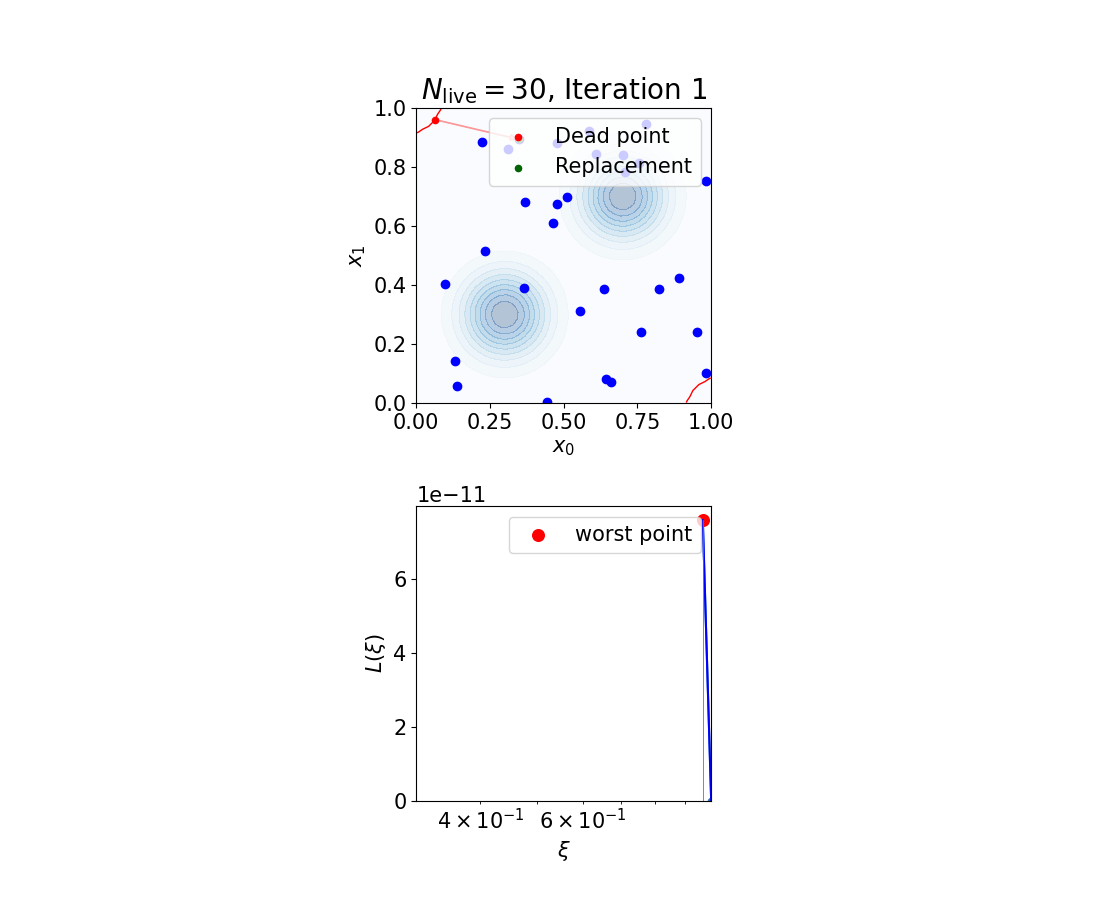
\includegraphics[width=\linewidth,
                             trim=240 20 250 50, clip]{assets/NS/nested_sampling_1.png}
            }

            % ----------- SHOW IMAGE 10 ON OVERLAY 2 -----------
            \only<2>{
            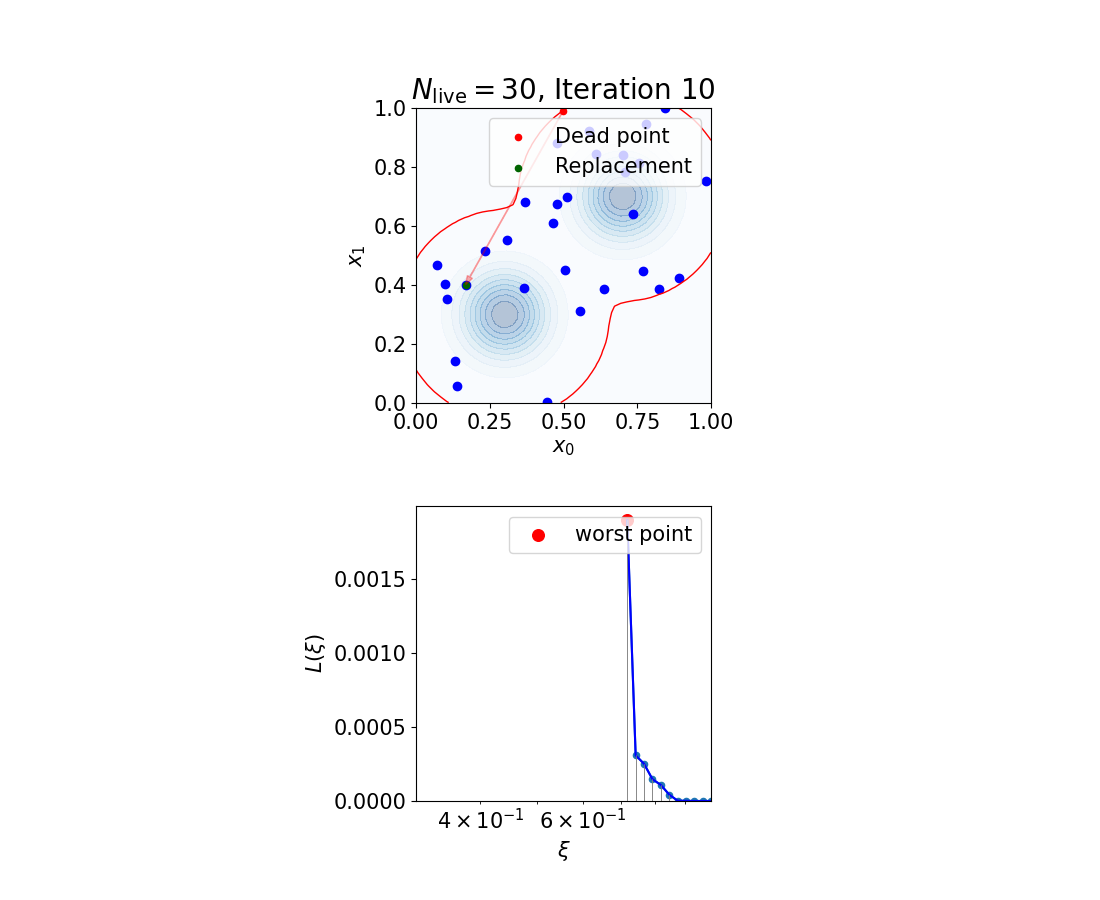
\includegraphics[width=\linewidth,
                             trim=240 20 250 50, clip]{assets/NS/nested_sampling_10.png}
            }

            % ----------- SHOW IMAGE 30 ON OVERLAY 3 -----------
            \only<3>{
            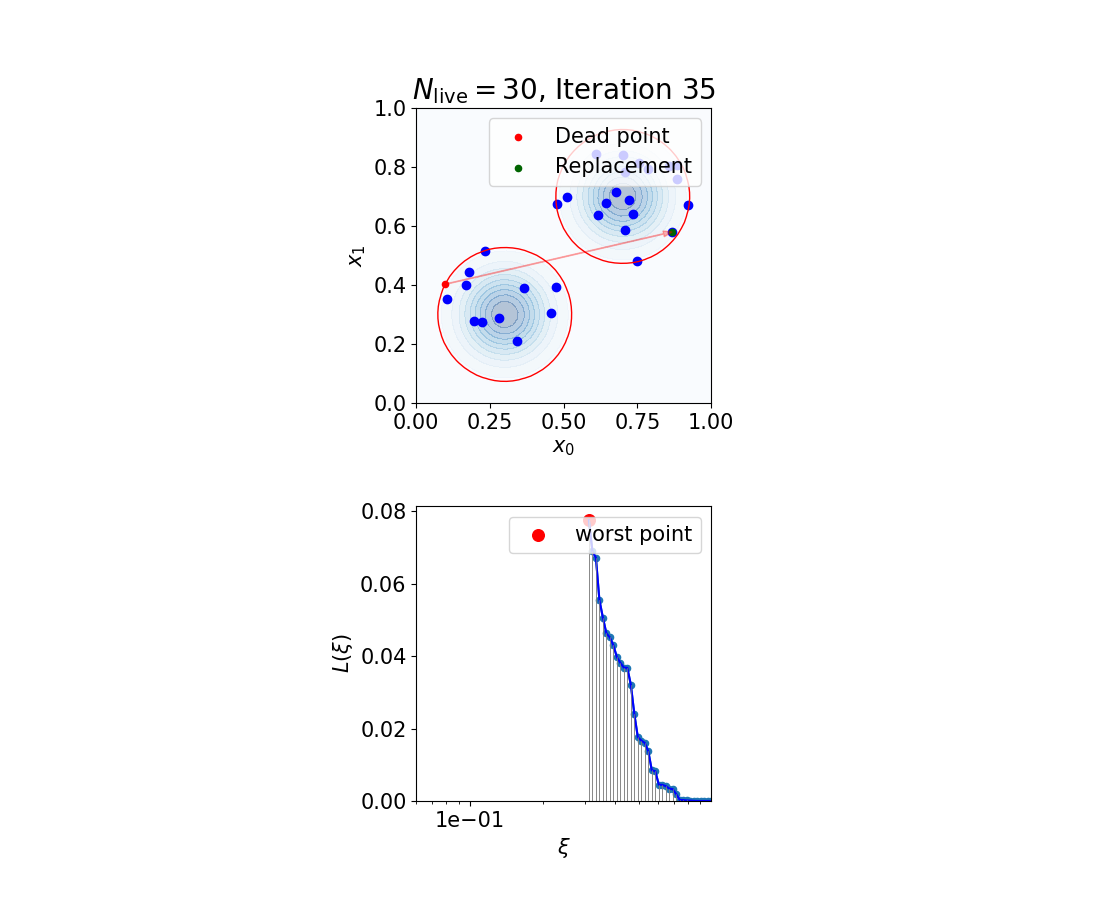
\includegraphics[width=\linewidth,
                             trim=240 20 250 50, clip]{assets/NS/nested_sampling_35.png}
            }
            \only<4>{
            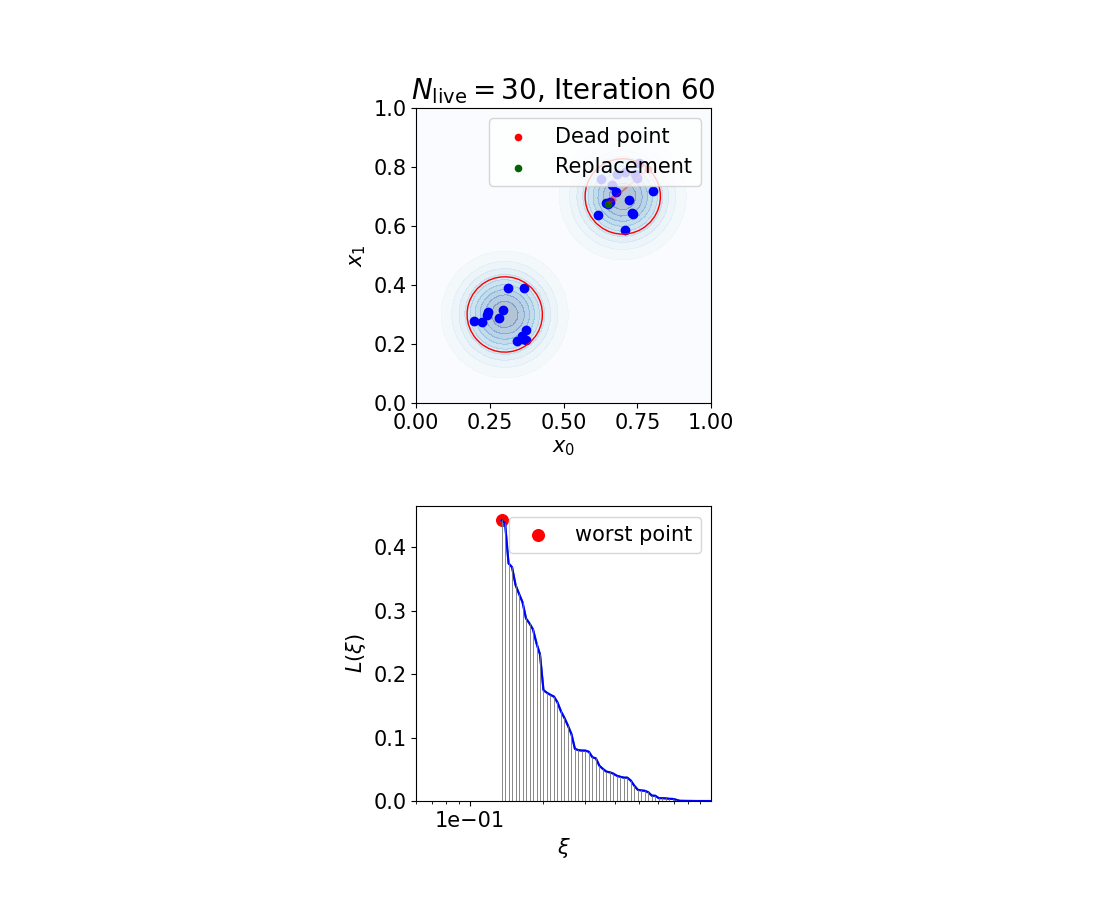
\includegraphics[width=\linewidth,
                             trim=240 20 250 50, clip]{assets/NS/nested_sampling_60.png}
            }
            \only<5>{
            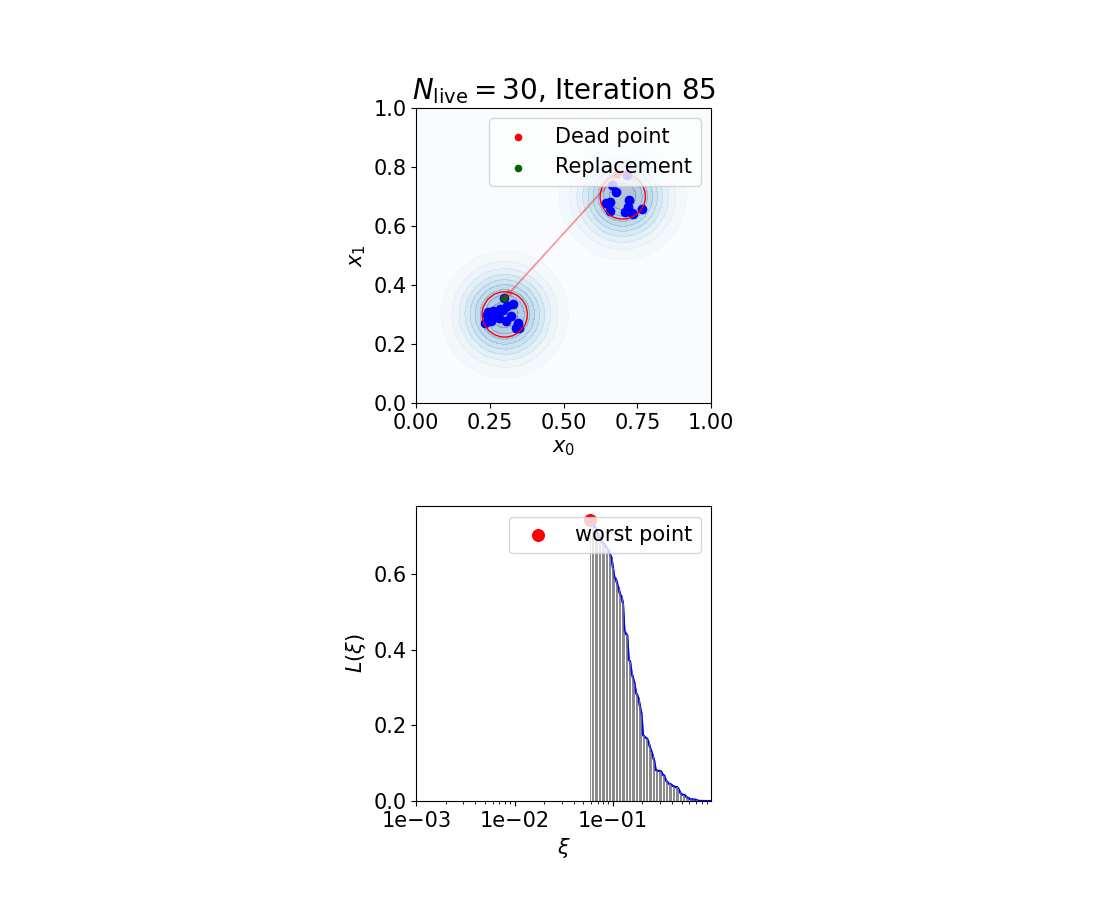
\includegraphics[width=\linewidth,
                             trim=240 20 250 50, clip]{assets/NS/nested_sampling_85.png}
            }
            \only<6>{
            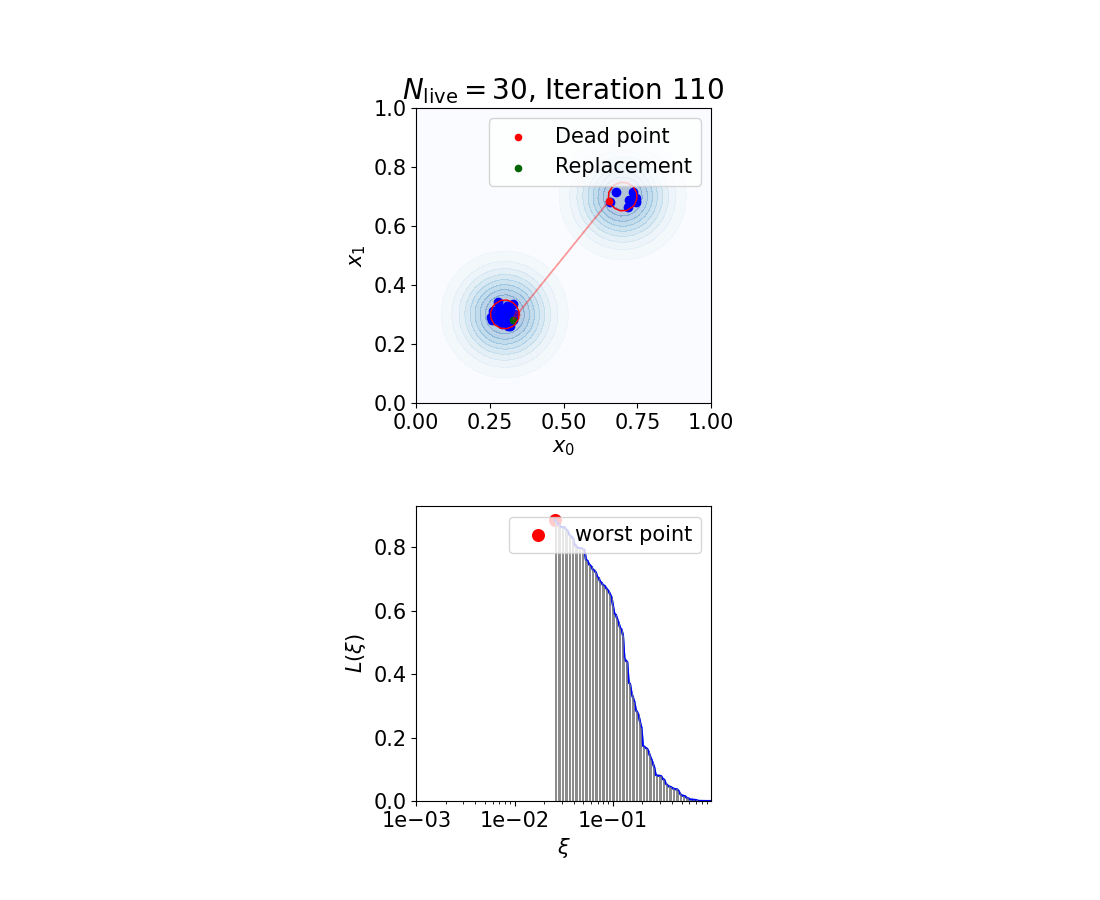
\includegraphics[width=\linewidth,
                             trim=240 20 250 50, clip]{assets/NS/nested_sampling_110.png}
            }
            \only<7>{
            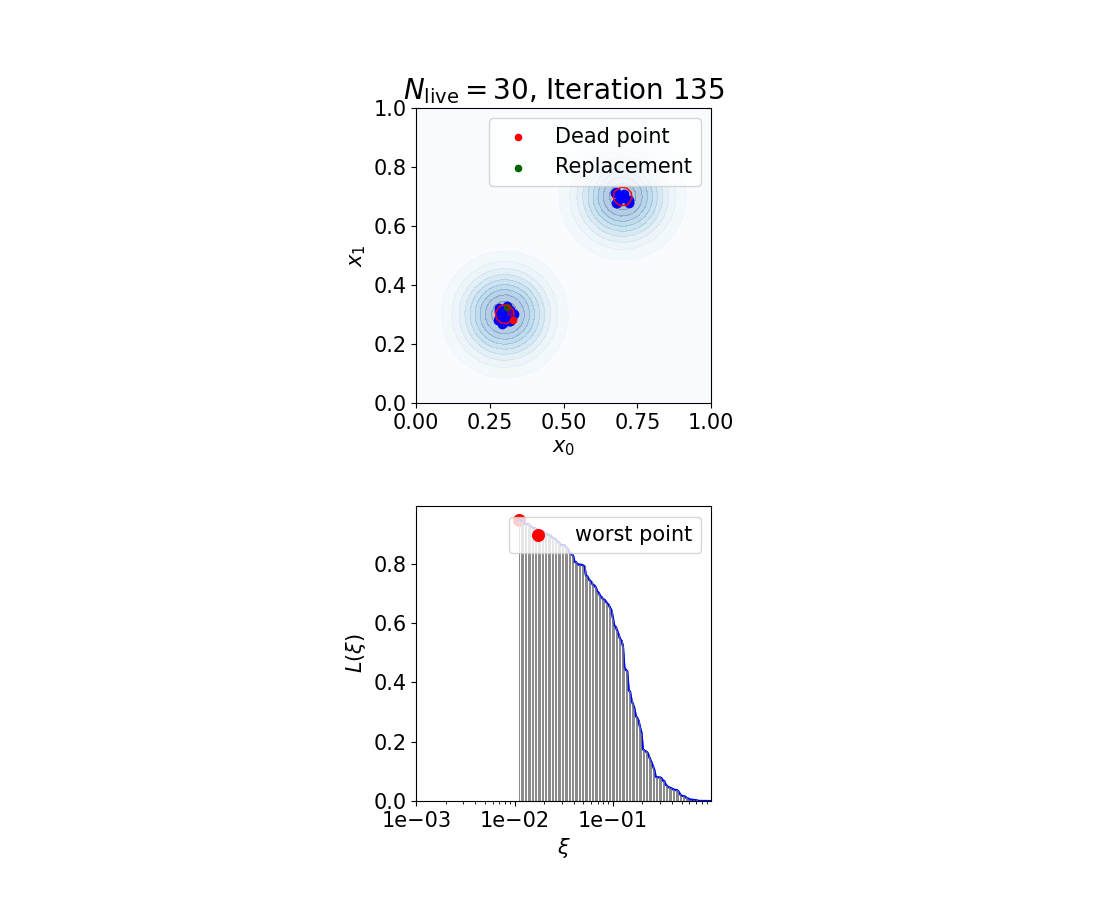
\includegraphics[width=\linewidth,
                             trim=240 20 250 50, clip]{assets/NS/nested_sampling_135.png}
            }
            \only<8>{
            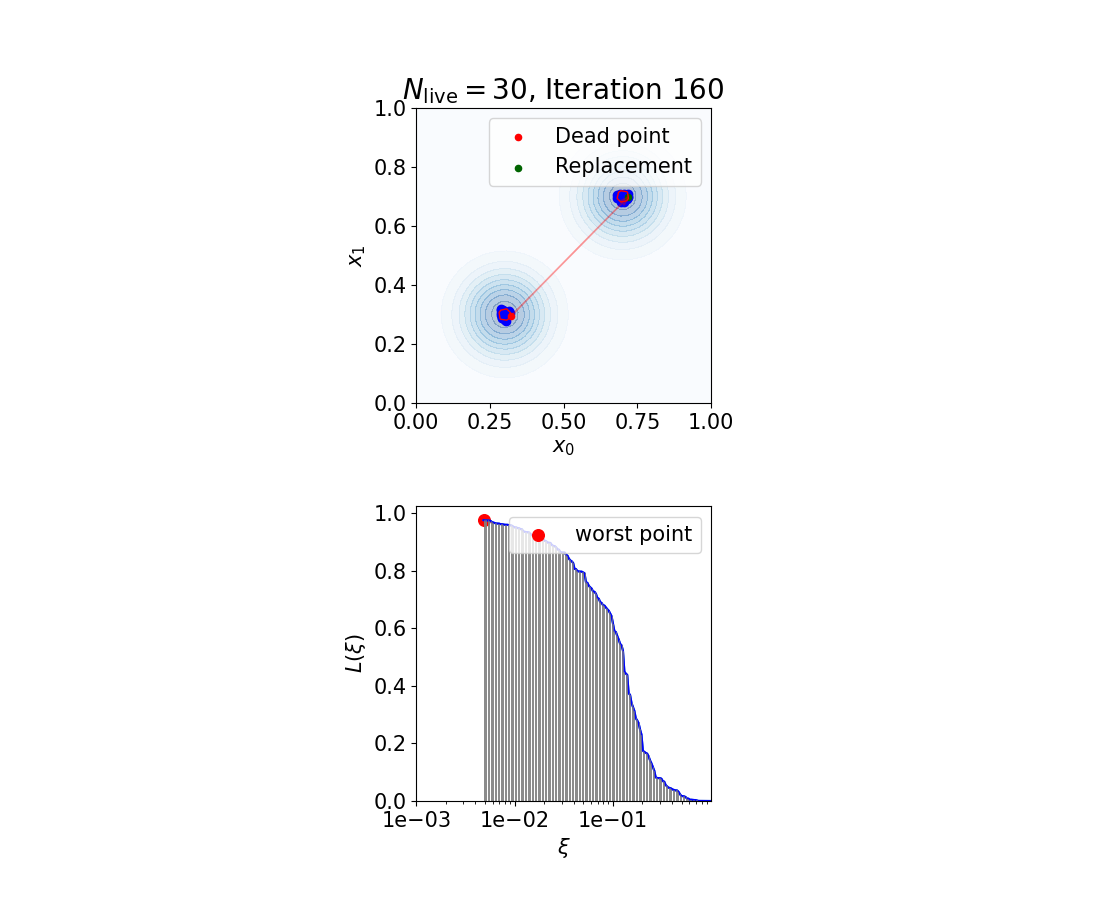
\includegraphics[width=\linewidth,
                             trim=240 20 250 50, clip]{assets/NS/nested_sampling_160.png}
            }
            \only<9>{
            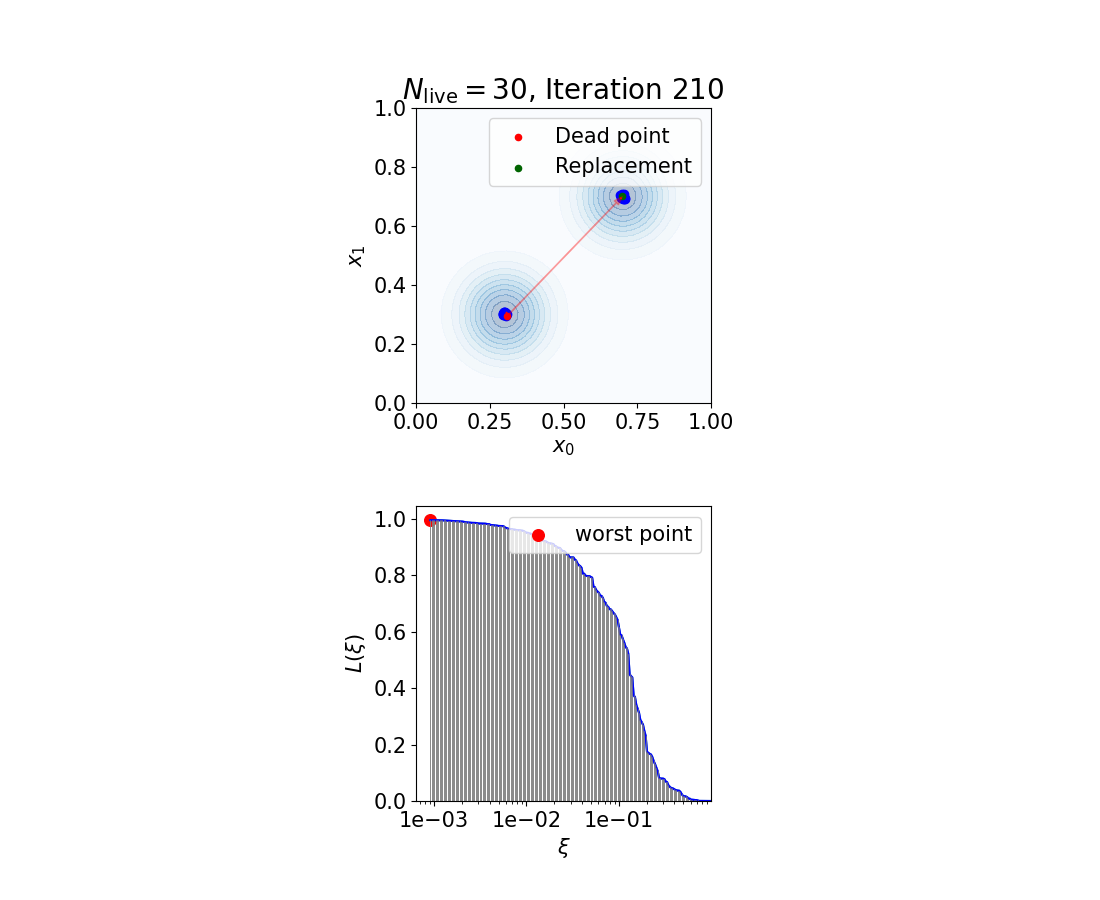
\includegraphics[width=\linewidth,
                             trim=240 20 250 50, clip]{assets/NS/nested_sampling_210.png}
            }
            \only<10>{
            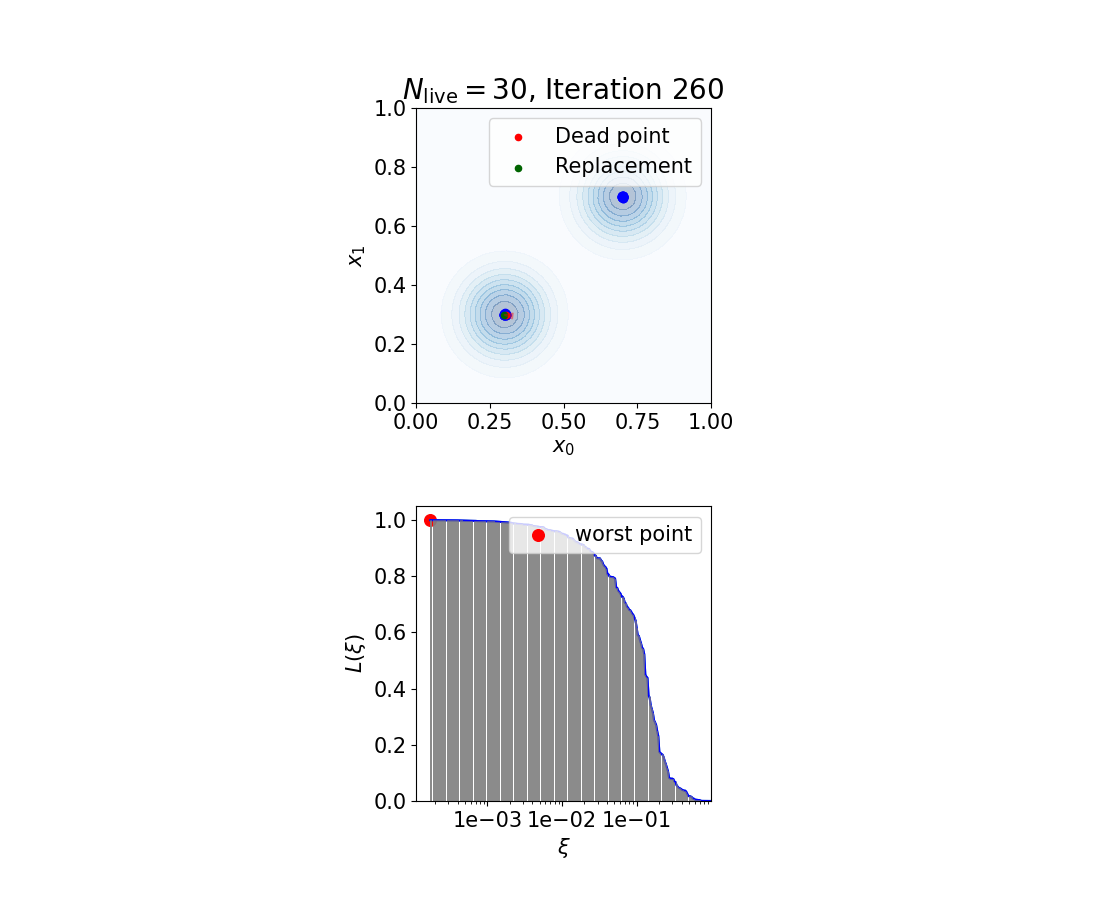
\includegraphics[width=\linewidth,
                             trim=240 20 250 50, clip]{assets/NS/nested_sampling_260.png}
            }

        \end{figure}
    \end{column}
\end{columns}

\end{frame}

\begin{frame}{Accelerated Nested Sampling}
\vspace{-0.5em}
\begin{columns}
    % ---------- LEFT COLUMN ----------
    \begin{column}{0.60\textwidth}
    \scriptsize
    \textbf{Traditional nested sampling (serial):}
    \begin{itemize}
        \item Remove one `worst' live point each iteration.
        \item New point conditioned on:
        \vspace{-1em}
        \[
        \mathcal{L} > \mathcal{L}_{\min}
        \]
        \item Inherently sequential MCMC slice samples
        \item \texttt{PolyChord - Handley et al 2025}
    \end{itemize}
    \vspace{1em}
    \par\noindent\rule{\linewidth}{0.35pt}
    \vspace{1em}
    \textbf{Accelerated nested sampling (parallel):}
    \begin{itemize}
        \item Discard a batch of $n_{\text{del}}$ `worst' points.
        \item All replacements conditioned on:
        \vspace{-1em}
        \[
        \mathcal{L}(\theta) > \mathcal{L}_{\min}
        \quad
        \mathcal{L}_{\min} = \max\{\mathcal{L}_1, \ldots, \mathcal{L}_{n_{\text{del}}}\}
        \]
        \item Sample each replacement independently \\ 
              \textcolor{red}{$\Rightarrow$ vectorised (vmap) across GPU}
        \item \texttt{Blackjax}
        \begin{itemize}
        \scriptsize
            \item \texttt{Cabezas at al 2024, Yallup et al 2025}
        \end{itemize} 
    \end{itemize}
 
    \end{column}

    % ---------- RIGHT COLUMN ----------
    \begin{column}{0.325\textwidth}
        \vspace{0.6em}
        \begin{figure}
            \centering

            % ----------- SHOW IMAGE 1 ON OVERLAY 1 -----------
            \only<1>{
            \vspace{-0.7em}
            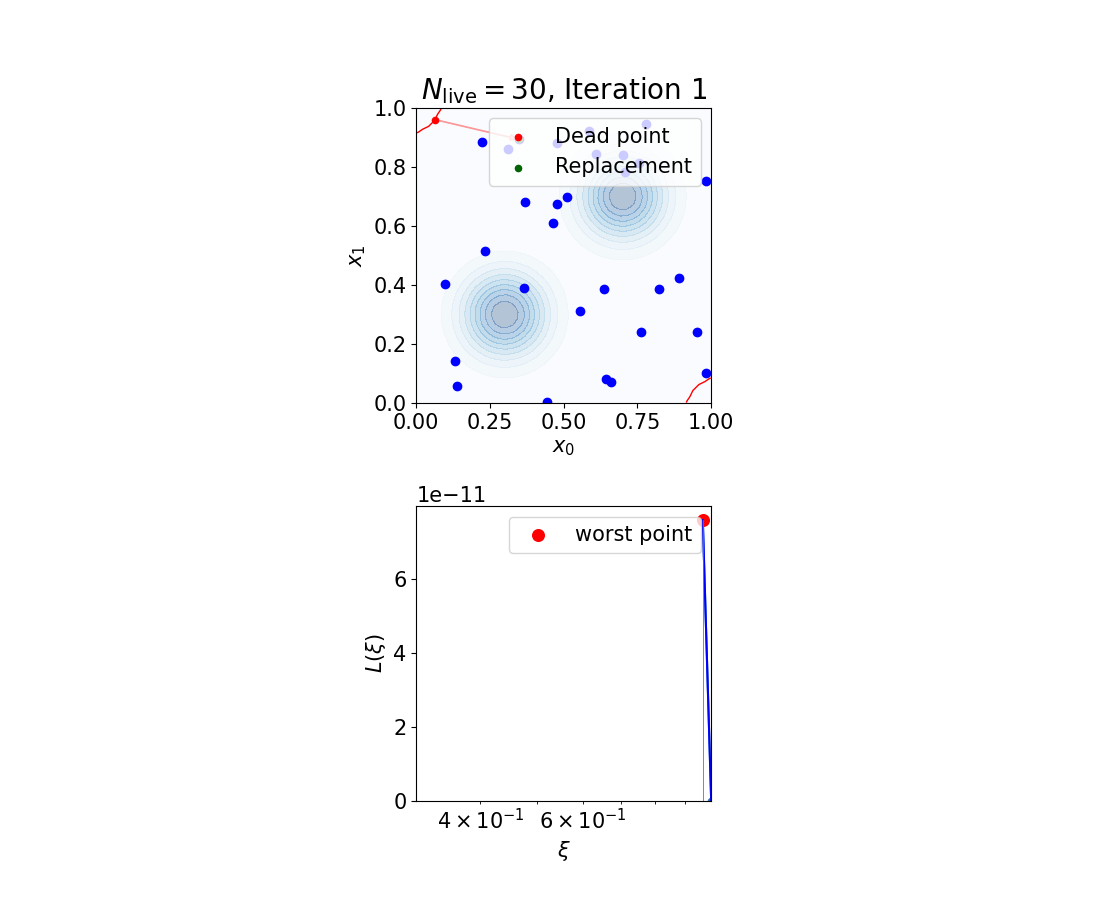
\includegraphics[width=\linewidth,
                             trim=240 300 250 40, clip]{assets/NS/nested_sampling_1.png}
            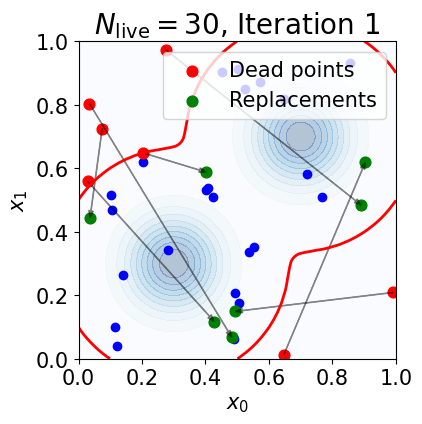
\includegraphics[width=0.9\linewidth]{assets/NS/parrallel_ns_1.png}
            }

            % ----------- SHOW IMAGE 10 ON OVERLAY 2 -----------
            \only<2>{
            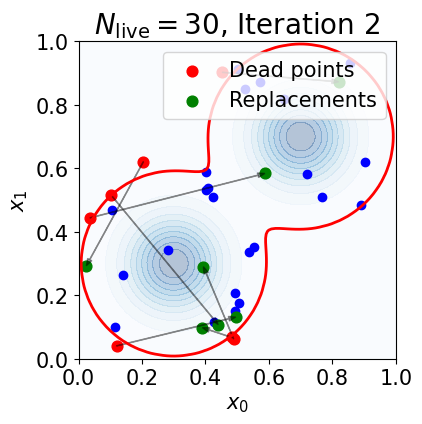
\includegraphics[width=0.9\linewidth]{assets/NS/parrallel_ns_2.png}
            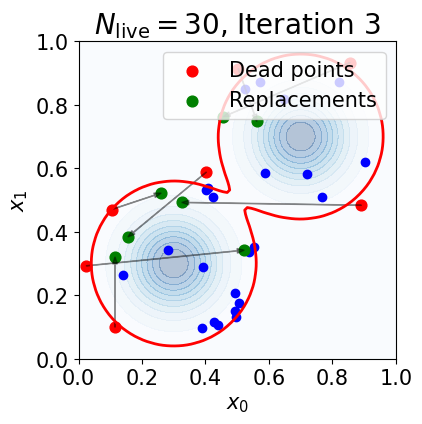
\includegraphics[width=0.9\linewidth]{assets/NS/parrallel_ns_3.png}
            }

        \end{figure}
    \end{column}
\end{columns}

\end{frame}

\begin{frame}{Workshop Summary}
\scriptsize
\textbf{Scientific Drivers}\\[0.25em]
\begin{itemize}\setlength\itemsep{0.15em}
    \item 21-cm cosmology demands high-dimensional inference over foreground, instrumental, and cosmological models across large datasets.
    \item LLM-era hardware and software investment is changing what is computationally feasible in science.
    \item In both REACH and BayesEoR Pipelines, GPU conversion is changing what is feasible in model complexity, data volume, validation, and financial cost.
    \item This applies both to simulation-based inference and to accelerating traditional Bayesian sampling.
\end{itemize}

\vspace{0.2em}
\textbf{Technical Enablers}\\[0.25em]
\begin{itemize}\setlength\itemsep{0.15em}
    \item Core stack: \texttt{JAX}, \texttt{XLA}, \texttt{BlackJAX}, \texttt{Optax}, \texttt{Flax}, \texttt{Distrax}
    \item Infrastructure: Google Compute Engine (\texttt{NVIDIA A100}), \texttt{AIRR} / \texttt{Isambard-AI} (\texttt{NVIDIA GH200})
\end{itemize}

\vspace{0.2em}
\textbf{Policy and Best Practice}\\[0.25em]
\begin{itemize}\setlength\itemsep{0.15em}
    \item Inference efficiency matters not only scientifically, but also financially and environmentally.
\end{itemize}
\end{frame}

\appendix


\end{document}
